% pcregrep --color='auto' -n '[^\x00-\x7F]' notes.bib
% biber notes

% \documentclass{tufte-book}
\documentclass[a4paper,11pt]{book}
\usepackage{a4wide}
\usepackage[unicode]{hyperref}
\usepackage[pdftex]{graphicx} % za slike
\usepackage{setspace}
\usepackage{textcomp}
\usepackage[version=3]{mhchem}
\usepackage{booktabs} % makes nice quality tables
\usepackage{emptypage}
\usepackage{palatino} 
\usepackage{pxfonts}
\usepackage{charter}

% \usepackage{natbib}
% \bibliographystyle{abbrvnat}
% \setcitestyle{authoryear,open={((},close={))}}

\usepackage{algorithm}
\usepackage[noend]{algpseudocode}
\makeatletter
% Reinsert missing \algbackskip
\def\algbackskip{\hskip-\ALG@thistlm}
\makeatother

\usepackage{amsopn}
\DeclareMathOperator*{\argmax}{\arg\,\max}

\renewcommand{\baselinestretch}{1.2}
\newcommand{\angl}[1]{(angl. {\em #1})}
\newcommand{\comment}[1]{#1}
\newcommand{\pd}[2]{\frac{\partial#1}{\partial#2}}
\newcommand{\plogp}[2]{{#1\over #2}\log_2{#1\over #2}}
\newcommand{\tr}{\intercal}
\newcommand{\mean}[1]{\overline{#1}}
\newcommand{\Var}{\mathrm{Var}}
\newcommand{\norm}[1]{\left\lVert#1\right\rVert}
\newcommand{\vect}[1]{\boldsymbol{#1}}
\newcommand{\matr}[1]{\boldsymbol{#1}}
\DeclareTextFontCommand{\emph}{\em}
\usepackage{xspace}
\def\etal{{\em et al.}\xspace}
\def\eg{{\em e.g.}\xspace}
\def\ie{{\em i.e.}\xspace}
\def\y{\vect{y}}
\def\b{\vect{\beta}}
\def\x{\vect{x}}
\def\X{\matr{X}}
\def\I{\matr{I}}

\DeclareMathOperator*{\argmin}{arg\,min}

\newcommand{\chaptersummary}[1]{ {\em #1}}

\usepackage{color}
\definecolor{light-gray}{gray}{0.95}
% \newcommand{\text}{\rm}
\usepackage{listings}
\usepackage{url}
% \usepackage{program}

\newtheorem{teorem}{Teorem}
\newtheorem{definition}{Definition}

\usepackage[most]{tcolorbox}
\newcounter{testexample}
\usepackage{lipsum}

\def\cost{{\rm cost}}
\def\R{\mathbb{R}}
\def\DS{\mathcal{D}}
\def\barwidth{3pt}
\def\exampletext{Example} % If English

\NewDocumentEnvironment{example}{ O{} }
{
\colorlet{colexam}{white!50!black} % Global example color
\newtcolorbox[use counter=testexample]{testexamplebox}{%
    % Example Frame Start
    empty,% Empty previously set parameters
    title={\exampletext: #1},% use \thetcbcounter to access the testexample counter text
    % Attaching a box requires an overlay
    attach boxed title to top left,
       % Ensures proper line breaking in longer titles
       minipage boxed title,
    % (boxed title style requires an overlay)
    boxed title style={empty,size=minimal,toprule=0pt,top=4pt,left=5mm,overlay={}},
    coltitle=colexam,fonttitle=\bfseries,
    before=\par\medskip\noindent,parbox=false,boxsep=0pt,left=5mm,right=0mm,top=2pt,breakable,pad at break=0mm,
       before upper=\csname @totalleftmargin\endcsname0pt, % Use instead of parbox=true. This ensures parskip is inherited by box.
    % Handles box when it exists on one page only
    overlay unbroken={\draw[colexam,line width=\barwidth] ([xshift=2pt]title.north west) -- ([xshift=2pt]frame.south west); },
    % Handles multipage box: first page
    overlay first={\draw[colexam,line width=\barwidth] ([xshift=-0pt]title.north west) -- ([xshift=-0pt]frame.south west); },
    % Handles multipage box: middle page
    overlay middle={\draw[colexam,line width=\barwidth] ([xshift=-0pt]frame.north west) -- ([xshift=-0pt]frame.south west); },
    % Handles multipage box: last page
    overlay last={\draw[colexam,line width=\barwidth] ([xshift=-0pt]frame.north west) -- ([xshift=-0pt]frame.south west); },%
    }
\begin{testexamplebox}}
{\end{testexamplebox}\endlist}


\NewDocumentEnvironment{summary}{ O{} }
{
\colorlet{colexam}{red!55!black} % Global example color
\newtcolorbox{summarybox}{%
    % Example Frame Start
    empty,% Empty previously set parameters
    % Attaching a box requires an overlay
    coltitle=colexam,fontupper=\bfseries,
    before=\par\medskip\noindent,parbox=false,boxsep=0pt,left=5mm,right=0mm,top=2pt,breakable,pad at break=0mm,
       before upper=\csname @totalleftmargin\endcsname0pt, % Use instead of parbox=true. This ensures parskip is inherited by box.
    % Handles box when it exists on one page only
    overlay unbroken={\draw[colexam,line width=\barwidth] ([xshift=2pt]frame.north west) -- ([xshift=2pt]frame.south west); },
    % Handles multipage box: first page
    overlay first={\draw[colexam,line width=\barwidth] ([xshift=-0pt]frame.north west) -- ([xshift=-0pt]frame.south west); },
    % Handles multipage box: middle page
    overlay middle={\draw[colexam,line width=\barwidth] ([xshift=-0pt]frame.north west) -- ([xshift=-0pt]frame.south west); },
    % Handles multipage box: last page
    overlay last={\draw[colexam,line width=\barwidth] ([xshift=-0pt]frame.north west) -- ([xshift=-0pt]frame.south west); },%
    }
\begin{summarybox}}
{\end{summarybox}\endlist}

\NewDocumentEnvironment{guide}{ O{} }
{
\colorlet{colexam}{yellow!55!black} % Global example color
\newtcolorbox{guidebox}{%
    % Example Frame Start
    empty,% Empty previously set parameters
    % Attaching a box requires an overlay
    coltitle=colexam,fontupper=\footnotesize,
    before=\par\medskip\noindent,parbox=false,boxsep=0pt,left=5mm,right=0mm,top=2pt,breakable,pad at break=0mm,
       before upper=\csname @totalleftmargin\endcsname0pt, % Use instead of parbox=true. This ensures parskip is inherited by box.
    % Handles box when it exists on one page only
    overlay unbroken={\draw[colexam,line width=\barwidth] ([xshift=2pt]frame.north west) -- ([xshift=2pt]frame.south west); },
    % Handles multipage box: first page
    overlay first={\draw[colexam,line width=\barwidth] ([xshift=-0pt]frame.north west) -- ([xshift=-0pt]frame.south west); },
    % Handles multipage box: middle page
    overlay middle={\draw[colexam,line width=\barwidth] ([xshift=-0pt]frame.north west) -- ([xshift=-0pt]frame.south west); },
    % Handles multipage box: last page
    overlay last={\draw[colexam,line width=\barwidth] ([xshift=-0pt]frame.north west) -- ([xshift=-0pt]frame.south west); },%
    }
\begin{guidebox}}
{\end{guidebox}\endlist}

\newcommand{\ifguide}[1]{\begin{guide}#1\end{guide}}
\renewcommand{\ifguide}[1]{}


\lstnewenvironment{python}[1][]{
\lstset{
language=python,
basicstyle=\ttfamily\footnotesize\setstretch{1},
stringstyle=\color{red},
showstringspaces=false,
alsoletter={1234567890},
otherkeywords={\ , \}, \{},
keywordstyle=\color{blue},
emph={access,and,break,class,continue,def,del,elif,else,%
except,exec,finally,for,from,global,if,import,in,is,%
lambda,not,or,pass,print,raise,return,try,while},
emphstyle=\color{black}\bfseries,
emph={[2]True, False, None, self},
emphstyle=[2]\color{green},
emph={[3]from, import, as},
emphstyle=[3]\color{blue},
upquote=true,
morecomment=[s]{"""}{"""},
commentstyle=\color{red}\slshape,
emph={[4]1, 2, 3, 4, 5, 6, 7, 8, 9, 0},
emphstyle=[4]\color{blue},
literate=*{:}{{\textcolor{blue}:}}{1}%
{=}{{\textcolor{blue}=}}{1}%
{-}{{\textcolor{blue}-}}{1}%
{+}{{\textcolor{blue}+}}{1}%
{*}{{\textcolor{blue}*}}{1}%
{!}{{\textcolor{blue}!}}{1}%
{(}{{\textcolor{blue}(}}{1}%
{)}{{\textcolor{blue})}}{1}%
{[}{{\textcolor{blue}[}}{1}%
{]}{{\textcolor{blue}]}}{1}%
{<}{{\textcolor{blue}<}}{1}%
{>}{{\textcolor{blue}>}}{1},%
% framexleftmargin=1mm, framextopmargin=1mm, frame=shadowbox, rulesepcolor=\color{blue},#1
}}{}

\lstset{ %
language=Python,
basicstyle=\ttfamily\setstretch{1},
backgroundcolor=\color{light-gray}
}

% include hyperlinks
\usepackage{hyperref}


% \usepackage[authordate,bibencoding=auto,strict,backend=biber,natbib]{biblatex-chicago}

\usepackage[
    backend=biber, natbib,
    style=authoryear,
]{biblatex}
\addbibresource{notes.bib}


\title{Machine Learning for Data Science 1 \\
\small (lecture notes, only for internal use)}
\author{Bla\v{z} Zupan, Erik \v{S}trumbelj}
\date{\today}


\begin{document}

\maketitle
\tableofcontents

\begin{refsection}
\chapter{Introduction}

\begin{summary}
Machine learning is a set of approaches that can detect patterns in the data. Types of machine learning include predictive and descriptive reinforcement learning. Two major classes of predictive learning are classification and regression. Examples of unsupervised learning approaches include principal component analysis, clustering, and dimensionality reduction. We can formalize predictive and descriptive learning as density estimation, where we develop probabilistic formulations of the form $p(y|\vect{x}_i,\mathcal{D})$ for predictive, and formulations of the form $p(y|\mathcal{D})$ for unsupervised learning. Resulting probabilistic models $p(y|\vect{\theta})$ or $p(y|\vect{x}_i; \vect{\theta})$ may include fixed number of parameters, or their number may vary according to the size of the training data. Interesting concepts in machine learning include the curse of dimensionality, inductive bias, overfitting, model selection, and absence of a universally best model that would fit all kinds of problem domains.~\footnote{These lecture notes follow Chapter 1 from~\citet{2012-Murphy}. Recommended additional reading is Chapter 2 from~\citet{ESL}.}
\end{summary}

\ifguide{
The purpose of this chapter is to introduce students to the basic definitions, general types of machine learning problems, things to consider in practical applications and fundamental concepts (curse of dimensionality, no-free-lunch theorem). We can also introduce kNN. Together with linear and logistic regression and PCA, which they already know, we have enough variety to cover the illustrative examples we need for this chapter.

Keep in mind that the Intro to DS course will already provide students with a practitioner's (black-box) understanding of the application of predictive models (classification/regression), clustering and dimensionality reduction, and dealing with missing values. This includes a black-box understanding of train/test and $k$-fold CV estimation of generalization error. Principles of Uncertainty will also give them a fundamental understanding of bootstrap non-parametric inference, maximum likelihood inference, Bayesian inference, and classical hypothesis testing. And a fundamental understanding of the following models: linear regression, logistic regression, PCA.
}

\section{The Purpose of Machine Learning}

\ifguide{
The students will already be used to the statistical notation of data, models (likelihoods), etc. ($y$, $x$, $p(y|x)$, etc.). It is important that the ML course continues with this to strengthen the student's abstraction. With a good understanding of $p(x,y)$ and $p(y|x)$ it becomes much easier to characterize terms that are commonly used in practice, such as classification, (un)supervised learning, regression, etc. (as we do below).
}

Machine learning is about learning models from data. More abstractly, given the training data $\mathcal{D}$, we would like to use the data to infer probability distributions. In other words, we would like to build models of the process $p(y)$ that generated the data.

The general task of learning $p(y|\mathcal{D})$, that is, inferring the conditional distribution of variables that define the processes given the data is very complex. In practice, we are, in most cases, not even interested in this general task. Instead, we are interested only in certain aspects of the distribution, and for these, apply specific types of machine learning, like classification, regression, or clustering.

In terms of applications, machine learning is a branch of artificial intelligence that provides algorithms that can automatically learn from experience without being explicitly programmed. While we will focus on theoretical aspects of machine learning, the reader of this text should place these in practical contexts and consider the tasks such as data acquistion, data cleaning, feature engineering, data cleaning and preprocessing, data visualisation, scoring and estimating the quality and utility of the developed models, and finally, their inclusion within working software and decision support systems. While practically of utmost importance, these engineering aspects will not be at the focus of this course.

\section{Types of Machine Learning}

\subsection*{Supervised learning}

Often, we are only interested in how a subset of variables is generated, while the remaining variables are used to explain the behavior of the variables of interest: $\{y_i, \vect{x}_i\}_{i=1}^n$. This is {\em supervised learning}, also known as {\em predictive learning} or {\rm predictions}. Here, $y$ is referred to as {\em response variable}, and $\vect{x}$ represents a vector of {\em features}. Depending on a branch of science that deals with machine learning, the dependent variable may also be referred to as a target variable, dependent variable (statistics), or label or class variable (machine learning). The independent variables are often referred to as covariates, independent variables, and predictors (statistics), or features and attributes (machine learning). Supervised learning starts with the training data, which includes $n$ pairs of instantiations of independent and dependent variables. The goal is to learn about $p(y|\vect{x})$ so that we can make predictions for future or unobserved values of independent variable $y$ for any combination of dependent variables $\vect{x}$ (see Table~\ref{tab:iris-sample}).

When $y$ is a nominal variable, we refer to this type of supervised learning as {\em classification}. When the nominal variable is two-valued, we deal with {\em binary classification}, and when the domain of the nominal variable includes three or more values, we refer to the problem as {\em multiclass classification}. When $y$ is continuous, we refer to the problem as {\em regression}. Less common cases consider a count or ordinal dependent variable, where we refer to the suitable approaches as {\em count regression} and {\em ordinal regression}, respectively. In most cases, the dependent variable $y$ will be a scalar, and we will refer to such cases as {\em univariate} classification or regression. When $y$ is a vector, we will refer to the problem as {\em multivariate} classification or regression.

Note that while various machine learning approaches specialize in a particular case, it is often easy to generalize a specific approach to deal with other types of the dependent variable. For instance, it is not difficult to adapt classification trees to the regression problems, or even to extend this approach to address multivariate learning.

\begin{table}
\caption{A small sample from the famous Iris data set, where Iris flowers are described with four numerical features and are labeled with Iris species. A possible task for this data set is supervised learning, with aim to build a model that predicts species from leaf morphology.}
\label{tab:iris-sample}
\begin{center}
\begin{tabular}{ccccl}
\toprule
sepal length & sepal width & petal length & petal width & iris \\
\midrule
4.4 & 2.9 & 1.4 & 0.2 & Iris-setosa \\
4.8 & 3.4 & 1.6 & 0.2 & Iris-setosa \\
5.4 & 3.9 & 1.3 & 0.4 & Iris-setosa \\
5.2 & 2.7 & 3.9 & 1.4 & Iris-versicolor \\
6.0 & 2.2 & 4.0 & 1.0 & Iris-versicolor \\
\bottomrule
\end{tabular}
\end{center}
\end{table}

\subsection*{Unsupervised learning}

We are using {\em unsupervised learning} when our problem does not include any response variable, that is, when the observations are not labelled. The goal of such learning is again to understand the data generative process $p(y)$, or at least to understand part of its structure.

A common approach to understanding the distribution $p(y)$ is to explain it with a smaller number of factors $\theta$, that is, to learn $p(y|\theta)$, effectively projecting the data into a lower-dimensional space. We refer to such procedure as {\em dimensionality reduction}. An extreme example of dimensionality reduction is {\em clustering}, when we try to explain $p(y)$ with a single nominal factor (see Fig.~\ref{fig:tsne-sc}). In essence, we are trying to group, or cluster, observations.

\begin{figure}[htbp]
\centering{\includegraphics[width=8cm]{figures/intro-tsne-single-cell.png}}
\caption{A two-dimensional visualisation of blood cells, originally described with expressions of thousands of features. The visualisation was constructed using t-SNE dimensionality reduction, and exposes potential clusters that need to be further analyzed.}
\label{fig:tsne-sc}
\end{figure}

\subsection*{Reinforcement learning}

Reinforcement learning is about learning actions of software agents in an environment where the goal is to maximize reward. An example of reinforcement learning is to learn the actions of a robot that travels through the maze and receives sensor input. A reward, in this case, could be time spent in a maze. Reinforcement learning is different from supervised learning in not requiring labeled input. Instead, reinforcement learning aims to find the balance between the exploration of uncharted territory and the exploitation of current knowledge. While we will focus on unsupervised and supervised learning in this course, we will only dive into reinforcement learning in one of our final sessions.


\section{Models and Learning}

A {\em model} $\mathcal{H}$ is in the most abstract sense a collection of distributions (densities, functions, ...). The elements of a model depend on our task.

\begin{example}[Simple linear regression - statistical model]
The simple linear regression is a set of densities \\
$\mathcal{H} =\left\lbrace p(y|\vect{x},\vect{\b},\alpha, \sigma)  = dnorm(\vect{\b}\vect{x} + \alpha, \sigma^2), \vect{\b}, \alpha \in \R, \sigma > 0 \right\rbrace$
\end{example}

\begin{example}[Simple linear regression - function approximation]
The simple linear regression is a set of functions
$\mathcal{H} =\left\lbrace f(\vect{x},\vect{\b},\alpha) = \vect{\b} \vect{x} + \alpha, \vect{\b}, \alpha \in \R \right\rbrace$
\end{example}

It is important to reinforce the view of a model as a set of hypotheses. Learning is the process of expressing a preference for certain hypotheses based on evidence (data). Choosing a particular machine learning algorithm, or in other words, choosing a particular model means expressing a preference for a certain type of hypothesis. The logistic regression model, in its basic form, will construct a model which will linearly separate the parameter space of the data instances to, prefarably, separate the data instances from either of the two classes. Separation plane constructed by classification trees may be much more complex and, implicitly, require many more parameters for its descriptions. The choice of the model also entails the choice of the complexity of the hypothesis, which in turn is related to the goodness of fit, overfitting, explainability, and other issues we expose in the text below.

A model is often also referred to as a hypothesis or set of hypotheses. Learning is often referred to as training the model, fitting the model/parameters, estimation.

{\em Learning} is the process of selecting elements of $\mathcal{H}$ based on some utility and using data. This is general. In practice, we can select a single element (a single density, function, distribution; as in the two function approximation examples above), a set of elements or even weight each element, for example, a distribution across all elements, as in Bayesian approaches.

Learning is in most cases just a problem in {\em computation} to be addressed through mathematical, numerical, algorithmic procedures. For parametric models, we typically do {\em least-squares} or {\em maximum likelihood} estimations to obtain {\em point estimates} of the parameters of the model. That is, by learning, we select a single model. Learning thus becomes an {\em optimization} problem, or {\em Bayesian inference}, which is an {\em integration} or optimization problem, if we do some sort of {\em structural approximation} or {\em MAP}. \


\subsection*{Parametric and Nonparametric Models}

If the set $\mathcal{H}$ can be parametrized with a finite number of parameters, we call the model {\em parametric}. Otherwise, it is {\em nonparametric}. A parametric model captures all information about the properties of the data within its fixed number of parameters. Predictions using non-parametric models require knowledge about the current state of the system, that is, require access to the current data.

\begin{example}[1-nearest neighbor model - a nonparametric model]
$\mathcal{H} = \lbrace$ all functions $f$ that can be expressed with a set of points (data instances) and the rule that $f(\vect{x}) = y_i$ of point $x$ nearest to $x_i$, according to a chosen distance metric$\rbrace$ (see Fig.~\ref{fig:1-nn})
\end{example}

\begin{figure}[htbp]
\centering{\includegraphics[width=0.6\linewidth]{figures/intro-knn-1.pdf}}
\caption{Decision boundary of a 1-nearest neighbor model trained on a two-featured binary classification data set with 380 data instances (170 in one class and 210 in the other) as shown on a figure. The decision boundary is complex and may substantially change with any addition on removal of the data.}
\label{fig:1-nn}
\end{figure}

Parametric models are easier to compute than non-parametric models. Non-parametric models are often more complex and grow with data. Parametric models depend on the data only through a finite number of parameters, while in non-parametric models, the complexity of the model depends on the training set. Researchers mostly prefer parametric models because it may be easier to estimate its parameters, easier to perform predictions, and easier to tell a story about the data according to a parametric model (e.g., sensitivity analysis, effects of the changes in parameters, parameter interactions). In this sense, parametric models are more prone to interpretation by domain experts. In parametric models, the parameter estimates may have better statistical properties compared to those of non-parametric regression.

Parametric models make stronger assumptions about the data; the learning may be successfull if these assumptions are valid, but the inferred predictors may fail if these assumptions are violated. Think of modeling a sine curve with a linear regression model. A non-parametric algorithm is computationally slower but makes fewer assumptions about the data. In (overly) simplified view, the trade-offs between parametric and non-parametric algorithms are in computational cost and accuracy.

Notice that non-parametric models are related to {\em lazy learning}. Lazy learning methods generalize the training data at the time of prediction. This type of learning is an alternative to {\em eager learning}, where the system tries to generalize the training data before receiving queries. An example of the lazy learner is a $K$-nearest neighbor algorithm. Lazy learners may have an advantage in real-time environments, where the training data changes in time and models trained in the past become obsolete in a relatively short time due to emergent new data and changes of the distributions and underlying processes that generated the data.

\ifguide{
It is good for the instructor to be aware that this definition of parametric models is operational but not rigorous. In fact, it is flawed. The set of all possible probability measures has the same cardinality as R. In other words, even a nonparametric model can be written as a model with a single real parameter. Assuming smoothnes solves the technical difficulties, but all of this is outside the scope of this course.
}

\section{Challenges of Applied Machine Learning}

\subsection*{Model Evaluation and Selection}

In theory, assuming uniform distribution over all possible datasets, there is no single best model. In fact, and again, in theory, no model is strictly better than any other model. This is in the literature referred to as {\em no free lunch theorem}, which states that any two optimization algorithms are equivalent when their performance is averaged across all possible problems~\citep{2005-Wolpert-Macready}. 

In practice, however, some characteristics are more common in datasets, so some models and algorithms perform better on average because their assumptions ({\em inductive bias}) better match the characteristics of the data generating process.

The above makes {\em model selection} a key part of applied machine learning. In order to train a model, we should define some measure of utility we would like to optimize. A trivial approach is then to select the model with the best utility on our available data. However, estimating the model's utility on the data it was trained on is biased and optimistic. In practice, the model's utility on the training data (so-called {\em in-sample} error) may be substantially better than on independent test data ({\em out-of-sample} error or {\em generalization error}). This effect is also known as {\em overfitting}, and it is something that we want to both detect and prevent.

\begin{figure}
\centering{
\includegraphics[width=0.47\linewidth]{figures/intro-knn-50.pdf}
\hfill
\includegraphics[width=0.47\linewidth]{figures/intro-logreg.pdf}
}
\caption{Decision boundary on a two-featured binary classification data set as inferred by nearest neighbor algorithm with K=50 and by logistic regression. Which model would perform better on new data?}
\label{fig:1-nn}
\end{figure}

\subsection*{Overfitting}

Overfitting occurs when machine learning model trained on a (limited) data set captures noise of the data instead of the underlying data generation processes. This modelling error occurs when an inferred hypothesis is too closely fit to a limited set of data points, or when a model is too complex for a given data (e.g., Fig.~\ref{fig:tree-overfit}). 

\begin{figure}[htbp]
\centering{\includegraphics[width=0.6\linewidth]{figures/intro-tree-10.pdf}}
\caption{Classification trees would often overfit the training data. Figure shows decision boundary of a tree where the allowed maximum tree depth was 10. The decision boundary is complex and often covers single-case exceptions.}
\label{fig:tree-overfit}
\end{figure}

\begin{figure}[htbp]
\centering{
\includegraphics[width=0.47\linewidth]{figures/intro-heatmap-default.pdf}
\hfill
\includegraphics[width=0.47\linewidth]{figures/intro-heatmap-fss.pdf}
}
\caption{Co-clustering of a random data set with 20 instances and 10 features (left), and co-clustering of a similar data set with 10000 features, of which 10 features were selected that best correlate with a binary label (right). Notice a clear pattern of colors and shades in the right heatmap, which should not be there if correct data preprocessing procedures were applied.}
\label{fig:heatmaps-overfitting}
\end{figure}

The related practical challenges include knowing when overfitting occurs and finding the right remedy for overfitting. Another challenge is to avoid modeling procedures that led to overfitting. None of these challenges is trivial, and beginners or even quite experienced practitioners often make mistakes that lead to overfitting and consequentially report over-optimistic scores for their modeling procedures. For instance, it has been found that some (if not most) of significant reports on the analysis of microarray gene expression data sets at the break of the century included overfitting~\citep{2003-Simon}. Common reported mistakes included feature selection before cross-validation or class label-informed feature selection before data visualization. Reports on good accuracies are, despite teachings in data science, present also in recent literature, as reported by \citet{2019-Vandewiele}. The authors examined reports on the analysis of a collection of electrohysterogram signals. There, related reports oversampled the data prior to cross-validation, and hence falsely obtained almost perfect accuracies.


\subsection*{Model Complexity and Effective Number of Parameters}

More complex models are more likely to overfit (see Figs.~\ref{fig:tree-depth-overfit} and \ref{fig:knn-learning-curve}), but the ``right'' complexity of the model may depend on the amount of data we have (see Fig.~\ref{fig:lr-overfitting}). In parametric models, especially linear models, the model's complexity easily be measured in terms of the number of parameters (or degrees of freedom). For nonparametric models the theory is more complex ({\em e.g.}, Vapnik–Chervonenkis dimension) and introduces the concept of the {\em effective number of parameters}. Typically, nonparametric models have a higher number of effective parameters and are thus able to better fit the data but also more prone to overfitting. But they are more difficult to interpret.

\begin{figure}[htbp]
\centering{\includegraphics[width=0.6\linewidth]{figures/intro-tree-overfit-depth.pdf}}
\caption{A classification tree accuracy on a random class-balanced binary classification data set with one feature and 50 data instances. Trees were grown to a specified maximal depth. More complex trees better fit the training data.}
\label{fig:tree-depth-overfit}
\end{figure}

\begin{figure}[htbp]
\centering{
\centering{\includegraphics[width=0.6\linewidth]{figures/intro-knn-learning-curve.pdf}}
}
\caption{A training and test-set tradeoff for $k$-nearest neighbor model. On the training data, the accuracy falls with raising $k$, while on the test data set the accuracy peaks at around $k=10$. Hyper-parameter estimation is one of the key issues when selecting the most appropriate model.}
\label{fig:knn-learning-curve}
\end{figure}


\begin{figure}[htbp]
\centering{
\centering{\includegraphics[width=0.6\linewidth]{figures/intro-lr-overfit-features.pdf}}
}
\caption{Logistic regression is more robust to overfitting than classification trees, but succombs as well when given sufficient number of features. A graph shows a training error on a random 50-instance binary classification data set when adding up to 35 features.}
\label{fig:lr-overfitting}
\end{figure}

\subsection*{Practical Utility of Machine Learning Models}

In practical applications, there are other dimensions (other than predictive accuracy, etc.) that we need to consider:

\begin{itemize}
\item {\em Computational aspects} include runtime complexity and resource consumption and are specifically relevant when modeling large data sets and streaming data, where models need to be adapted frequently and where there is inherent concept drift. Notice that while some computational can be mitigated with modern hardware, but we must understand that even taking into account pairwise feature interactions requires computation squared in the number of features, not even counting the number of data points. All alternatives are based on discarding some information: data subsampling (sublinear learning algorithms), feature selection, or discarding higher-order feature interactions.
\item {\em Implementation aspects}, where data scientists need to decide which parts of the analysis procedures to implement on their own, gaining in flexibility, and for which to rely on already existing implementations. These later may also be limited in terms of data type (e.g., sparse or full), scalability (multi-core, multi-processor, or multi-GPU computing), and data access (e.g., Excel tables, SQL databases, or data in the cloud).
\item {\em Interpretability}, which often refers to the question if the model is readable, or can it be converted to a readable format. And if it is readable, is its interpretation easy (e.g., just a few if-then-rules) or impossible (e.g., a long list of rules, or a large classification tree).
\item {\em Explainability}, often confused with interpretability, places a model within a context of a problem domain and asks a question did we gain any new knowledge. To achieve explainability, one would often need to combine the interpretation of the model with extra formalized knowledge about the domain ({\em e.g.}, feature groups, ontologies, rules, and similar).
\end{itemize}

Every modeling paradigm we introduce in this course should and will be discussed from these perspectives. Notice that most data science courses often focus on predictive accuracy alone; the intended audience may often forget that in practice, other issues are equally or even more important.

\subsection*{Curse of Dimensionality}

In practice, the complexity of the models we want to fit is not bound only by computational resources but also the fact that a linear increase in the number of variables can result in exponential increases in the number of possible configurations. Therefore, the amount of data that would be required to distinguish between these configurations is impractical. 

The curse of dimensionality may also inhibit, or even cripple some machine learning methods. For instance, $k$-nearest neighbors may work well on two-dimensional data, but as soon as the number of dimensions increases, to a few more dimensions, the algorithm fails. To illustrate this point, consider embedding a small $d$-dimensional cube of side $s$ inside a larger unit cube (Fig.~\ref{fig:cube-in-cube}). Let the data be uniformly distributed within the unit cube. Suppose we estimate the density of a class labels around a test point $\vect{x}$ by growing a smaller hyper-cue until it contains a desired fraction $f$ of the data points. The expected length of this cube will be $s(f,d)=f^{1/d}$. Say, with $d=10$ and to base our estimate on $10\%$ of the data, the length of the smaller cube would need to be $s=0.8$. The approach, despite the name ``nearest neighbor'' is no longer very local, as even with the modest feature sizes, it relies on data points that are far away. Even with $1\%$ coverage, the size of the small cube needs to be substantial, as $s(0.01,10)=0.63$. With a number of features growing, we quickly have to start taking into account points that are not close or risk increasing variance.

\begin{figure}[htbp]
\centering{
\centering{\includegraphics[width=0.8\linewidth]{figures/intro-cube-overfitting.png}}
}
\caption{We embed a small cube within a unit cube (left) and assess a lenght of the edge of a small cube to cover a fraction of uniformly spread data. Graphs borrowed from~\citet{2012-Murphy}.}
\label{fig:cube-in-cube}
\end{figure}


\printbibliography[heading=subbibliography]
\end{refsection}
\begin{refsection}
\chapter{Trees and Forests}

\begin{summary}
Trees introduce learning via recursive partitioning of the input variable space. Depending on the learning task, the algorithm used is either a classification tree or a regression tree, respectively. The inference of trees is fast but leads to models that are not stable and have high variance. To reduce the variance and increase stability, the upgrade of the tree-learning approach may construct a set of trees. We define two such procedures; one called bootstrap aggregation (bagging) and the other random forest.
\end{summary}

\section{Classification and Regression Trees (CART)}

Classification and regression trees, somehow surprisingly, conceptually relate to other advanced machine learning approaches, such as kernel methods, generalized linear models, and adaptive basis function models. While we have yet to discuss them, let us visit them briefly for some motivation. The (generalized) linear modeling paradigm, as introduced in the next lecture, assumes that we can interpret the data generating process with a family of distributions whose parameters are in a (transformed) linear relationship with the input variables. These are parametric models. For kernel methods, the prediction takes the form of a weighted sum $f(\vect{x})=\vect{w}^\tr\vect{\phi}(\vect{x})$, where $\vect{w}$ is a weight vector and $\phi$ is a vector of similarities with an input example $\vect{x}$, such that
$$ \vect{\phi}(\vect{x}) = [\kappa(\vect{x},\vect{\mu}_1), \ldots, \kappa(\vect{x},\vect{\mu}_n)] $$
where $\vect{\mu}_k$ represents either all the training data or some sample, and $\kappa$ is a kernel function. Kernel functions are, in general, defined in advance, and coming up with a good kernel is hard and may depend on the problem domain.

Learning kernel functions is on option, but is computationally expensive and requires a lot of data. An alternative approach is to forget about kernels, and instead infer useful features $\vect{\phi}(\vect{x})$ directly from the training data. This is an approach used by adaptive basis function model, which takes the form
$$ f(\vect{x})=w_0+\sum_{m=1}^{M} w_m\phi_m(\vect{x}) $$
where $\phi_m(\vect{x})$ is the $m$-th basis function inferred from the training data. The basis functions are parametric, so that we can write $\phi_m(\vect{x})=\phi_m(\vect{x};\vect{v}_m)$, where $\vect{v}_m$ are the parameters of the basis function itself. The CART approach can be viewed as a special case of adaptive basis function model. CART recursively partitions the input space and defines a simplified local model in each resulting region. Recursive partitioning can be represented as a tree, where partitioning conditions are stored in internal nodes and region models in the leaves. The model takes the following form
\begin{align}
f(\vect{x}) & = \mathbb{E}[y|\vect{x}] \\
 & = \sum_{m=1}^M w_m \mathbb{I}(\vect{x}\in R_m) \\
 & = \sum_{m=1}^M w_m\phi(\vect{x};\vect{v}_m)
\end{align}
where $R_m$ denotes the $m$'th region and $w_m$ is, simplified, the main response in the region. The set $\vect{v}_m$ encodes the choice of the variable to split on and the related threshold value in the path from the root of the tree to the specific leaf. Notice that in CART the regions do not overlap, and that the training example falls in only and exactly one of the constructed regions. The region splits are defined on exactly one of the variables and are thus axis parallel.

\subsection*{Basic Idea}

From the viewpoint of model construction and compared to generalized linear models, kernel methods, and inference of adaptive basis function models, CART introduces a fundamentally different modeling paradigm. One that assumes that we can interpret the data generating process as a partition of the input variable space into homogeneous (pure) regions -- regions where there is little or no uncertainty left about the target variable. For regression, the target variable for the data instances within this region is almost constant (see Fig.~\ref{fig:trees-sin}). For classification, a majority of data instances in the region have the same value of the target variable.

\begin{figure}
\centering{
\includegraphics[width=0.47\linewidth]{figures/trees-sin-1.pdf}
\hfill
\includegraphics[width=0.47\linewidth]{figures/trees-sin-2.pdf}

\includegraphics[width=0.47\linewidth]{figures/trees-sin-3.pdf}
\hfill
\includegraphics[width=0.47\linewidth]{figures/trees-sin-4.pdf}
}
\caption{Regression trees fitted on data generated by a sine function with some noise. While the tree adapts well to the training data, its ability to overfit the training data is visible already with trees with of maximum depth of 4 (lower right).}
\label{fig:trees-sin}
\end{figure}

\begin{figure}[htbp]
\centering{\includegraphics[width=0.7\linewidth]{figures/trees-rtree}}
\caption{A regression tree with maximum depth of 2 from the data from Fig.~\ref{fig:trees-sin}.}
\label{fig:fig:trees-sin-2}
\end{figure}

\subsection*{The CART Algorithm}

Finding the optimal partitioning of the input variable space is in general NP-complete, even if using axis-parallel splits only. That is, it is infeasible to check all possible partitions. Instead, we will consider a greedy algorithm (CART) that uses binary recursive partitioning of the input space, at each step choosing the best possible split (according to some pre-selected criterion). Notice that this algorithm does not use any look-ahead, and while there are published studies of such algorithms, they have found no use in practice. Algorithm~\ref{alg:cart} shows the pseudocode of a CART algorithm.

\begin{algorithm}
\begin{algorithmic}[1]
\Procedure{fitTree}{$\DS$}
\State $(\DS_L, \DS_R, criterion) \gets split(\DS)$
\State $node \gets createNode(criterion, \DS)$
\If {stoppingCriterionMet(criterion, $\DS$)} \Return node \EndIf
\State $node.L \gets fitTree(\DS_L)$
\State $node.R \gets fitTree(\DS_R)$
\State \Return node
\EndProcedure
\end{algorithmic}
\caption{CART}\label{alg:cart}
\end{algorithm}

The CART algorithm uses several functions that require explanation:
\begin{itemize}
\item {\em createNode()}: This function creates an object that represents a tree node, which essentially stores the criterion that splits the data in a node and a possible reference to the data instances that are pertinent to the node. If the procedure finds a suitable node split, the node stores the information on its to siblings. Note that, as introduced above, the CART algorithm would construct binary trees.
\item {\em split()}: The assumption here is that features are numerical or at least ordinal. We order every feature based on possible splits (based on unique values in the data, so we have a finite number of possible splits). And then, we go through all possible feature-split combinations to find the one that is optimal according to our splitting criterion -- the one that minimizes the sum of the cost of the left and right subtrees. Below we discuss possible splitting criteria.

\item {\em stoppingCriterionMet()}: The stopping condition, also referred to as {\em pre-prunning} of the trees, can be one or more of the following:
\begin{itemize}
\item The partition is sufficiently homogeneous/pure. In particular, there is no point in splitting further if we have perfect homogeneity (all observations have the same value).
\item The gain $\Delta$ of splitting the data set in the current node (relative to stopping criterion) is below some pre-determined threshold, where
$$ \Delta = \cost(\DS) = \cost(\DS)-\left({|\DS_L|\over |\DS|}\cost(\DS_L) + {|\DS_R|\over |\DS|}\cost(\DS_R)\right)$$
\item The algorithm has reached pre-determined maximum tree depth.
\item Splitting the data set in the node would yield a leaf with number of observations below some pre-determined minimum.
\end{itemize}
\end{itemize}


\subsection*{Choice of the Splitting Criterion}

At each internal node, the inference method for the trees splits the training data set $\DS$ pertinent to the node to maximize some splitting criterion. The split uses a single feature from the training data set and forms a condition on the value of this feature that evaluates to true or false. The condition splits the data $\DS$ to two data sets, each pertinent to one of the two siblings of the node. The result is a binary tree. Notice that we could use other, non-binary, splitting mechanisms, but they would lead to over-fragmentation of the data, increase the variance, and lead to increased overfitting.

Splitting criteria are related to data set purity, costs, loss, or estimated errors. They have to address the type of the target feature, this being either numerical or discrete. Note that the literature investigates many different criteria, and while, at least on the surface, these take different forms, the practical differences regarding overall accuracies and ordering of the features are often neglectable. The costs of the splitting is most often estimated for each of the resulting siblings (leaves), and then weighted according to the estimated probability that the data instance will fall in one of the two constructed regions
$$ \cost(node, criterion) = {|\DS_L|\over |\DS|}\cost(\DS_L) + {|\DS_R|\over |\DS|}\cost(\DS_R) $$

For regression trees, the most often used splitting criterion is the mean squared error of predicting with the subtree mean
$$ cost(\DS) = \sum_{i\in\DS}(y_i-\overline{y})^2 $$
where $\overline{y} = {1\over|\DS|}\sum_{i\in\DS}y_i$ is the mean of the target variable in the resulting data set.

Many more splitting criteria were proposed for the classification setting, and most of them rely on estimating class-conditional probabilities
$$ \hat{\pi}_c = {1\over|\DS|}\sum_{i\in\DS}\mathbb{I}(y_i\equiv c) $$
For instance, we can measure the {\em entropy} (or {\em deviance}) of the resulting data set
$$ \mathbb{H}(\hat{\vect{\pi}}) = -\sum_{c=1}^C \hat{\pi}_c \log \hat{\pi}_c $$
or can measure the expected error rate in the form of a {\em gini index}
$$ \sum_{c=1}^C \hat{\pi}_c (1-\hat{\pi}_c) = \sum_c \hat{\pi}_c - \sum_c \hat{\pi}_c^2 = 1 - \sum_c \hat{\pi}_c^2 $$
where $\hat{\pi}_c$ is the probabilty a random entry in the leaf belongs to class $c$, and $1-\hat{\pi}_c$ is the probability for this entry to be misclassified. Other criterion may include information gain, information gain ratio, chi-squared test, and similar. Note that with all the above criteria, splitting the training data set will never decrease the quality (and increase the cost) and in the worst case the quality will remain the same if the node's data set is already homogeneous. Notice that we are estimating all the costs on the training set and thus potentially overfitting the data.

\subsection*{Discussion}

There are several issues with growing and using the classification and regression trees. The trees have some advantages and many disadvantages. While, on their own, the trees are rather mediocre predictors, their enhancements in terms of ensembling discussed in the following sections of this chapter elevate them to at least a formidable baseline, if not state-of-the-art approach. Therefore, let us first review some of the issues that are pertinent to the development and utility of CART, that is, induction of single trees.

\begin{description}
\item[Interpretation.] Decision trees are easy to interpret. In fact, according to the current research, the interpretability of trees is only behind decision tables and individual rules when it comes to non-expert users. Yet, the standard decision tree algorithms are very susceptible to small changes in the inputs. A small change in the training data set can result in a substantially different tree. What good is an in-depth interpretation of the model if this is inherently unstable? We can mitigate instability by using bootstrapping to check if the algorithm produces stable trees before proceeding with the analysis. Also, learning a (stable) tree that mimics a more complex model such as a tree ensemble and neural networks is one of the most common approaches to explaining how the complex model works. This approach, though, has gained recent criticism that if one is after the explanation, one should primarily build interpretable models in the first place, and not represent complex models with simple ones~\citep{Rudin2019}.

\item[Low computational complexity.] Trees are fast to training and very fast in prediction. They scale well to large data sets. The only exception to this observation is in treatment of sparse data, that is, data with many unknown values. A thorough treatment of unknown values may invalidate the divide-and-conquer approach with the passing of full data sets to leaves and potentially visiting the entire tree when predicting. A potential remedy of this side effect is to impute the missing values before training or prediction.

\item[Weak inductive bias.] Compared to more sophisticated methods, including ensembles of trees and neural networks, classification and regression trees have a relatively weak inductive bias. That is, they will not perform the best (or close to) in terms of predictive quality on most practical problems. The two main issues are a {\em lack of smoothness} and {\em difficulty of capturing additive relationships}. See~\citep{ESL} for further details.

\item[Possible complex treatment of categorical input variables.] When splitting a predictor having $q$ possible unordered values, there are $2^{q-1}-1$ possible partitions of the $q$ values into two groups and the computations become prohibitive for large $q$. For example, consider the treatment of postal codes in the data sets. There are possible heuristic approaches to cope with such cases, though. For binary target variables, we can order the predictor classes according to the proportion falling in outcome class 1. Then we split this predictor as if it were an ordered predictor. One can show this gives the optimal split, in terms of cross-entropy or Gini index, among all possible splits. This result also holds for a quantitative outcome and squared error loss—the categories are ordered by increasing the mean of the outcome. The proof for binary outcomes is given by \citet{Brieman1984} and \citet{Ripley1996}; the proof for quantitative outcomes can be found in \citet{Fisher1958}. For multicategory outcomes, no such simplifications are possible, although various approximations have been proposed~\citep{Loh1988}.

The partitioning algorithm tends to favor categorical features with many values; the number of partitions grows exponentially in $q$, and the more choices we have, the more likely we can find an (arbitrarily) good one for the data at hand. This can lead to severe overfitting if $q$ is significant, and such variables should either be avoided or some preprocessing by means of a grouping of similar feature values, such as clustering, should be used. Also, note that dummy (one-hot) encoding of categorical variables can lead to the opposite problem of individual binary variables not being selected over many features represented encoded variables.

\item[The benefits of binary splits.] Rather than splitting each node into just two groups at each stage, we might consider multiway splits into more than two groups. While this can sometimes be useful, it is not a good general strategy. The problem is that multiway splits fragment the data too quickly, leaving insufficient data at the next level down. Hence we would want to use such splits only when needed. Since multiway splits can be achieved by a series of binary splits, the latter is preferred.

\item[treatment of missing values.] Suppose our data has some missing predictor values in some or all of the variables. We might discard any observation with some missing values, but this could lead to severe depletion of the training set. Alternatively, we might try to fill in (impute) the missing values, with say the mean of that predictor over the non-missing observations. For tree-based models, there are two better approaches. The first is applicable to categorical predictors: we make a new category for “missing.” From this, we might discover that observations with missing values for some measurement behave differently than those with non-missing values. The second more general approach is the construction of surrogate variables. When considering a predictor for a split, we use only the observations for which that predictor is not missing. Having chosen the best (primary) predictor and split point, we formed a list of surrogate predictors and split points. The first surrogate is the predictor and corresponding split point that best mimics the split of the training data achieved by the primary split. The second surrogate is the predictor and relevant split point that does second best, and so on. When sending observations down the tree either in the training phase or during prediction, we use the surrogate splits in order, if the primary splitting predictor is missing. Surrogate splits exploit correlations between predictors to try and alleviate the effect of missing data. The higher the correlation between the missing predictor and the other predictors, the smaller the loss of information due to the missing value.

\item[Tree pruning.] If the tree is allowed to grow until the leaves are entirely (or nearly) homogenous, we are likely to be overfitting. In some cases that is desirable - we will see such an example later with random forests, where we want an individual tree in the ensemble to include little modeling bias. However, in most cases, it is not. To prevent overfitting, we can carefully tune the stopping criteria. However, growing the entire tree and then post-processing it by {\em pruning} individual branches can sometimes lead to better results. The basic idea is to go over each split and check if not making that split would not result in a significant increase in error.
Additionally, we can use cross-validation to prune based on an estimate of the generalization error, making the process more robust. Note that cross-validation could (should), in theory, also be used when growing the tree. The reason why we make splits based on what is essentially training set error is that cross-validation would be computationally infeasible in most practical scenarios.

\item[Model trees.] As an alternative to reporting on average values in tree leaves, we can use non-trivial models. Many approaches combine trees with generalized linear (additive) models in the leaves. This can lead to improved results in problems that are a combination of crisp rules and (local) linear behavior while retaining most of the interpretability. However, it comes at the cost of computational complexity because it requires a more complex model evaluation when splitting the tree.

\item[Oblique feature space splitting.] Axis-parallel partitioning**: Most tree-based algorithms (including the one described above) limit themselves to axis-parallel splits. This can lead to very complicated trees if the boundaries between homogeneous regions do not follow this assumption. As an alternative, non-axis-parallel (oblique) algorithms have been developed. However, this comes at the cost of interpretability and computational complexity.
\end{description}

\section{Bagging}

Before we proceed with random forests, we will first introduce a component of random forests that has more general applicability. {\em Bagging} (Bootstrap Aggregation) is a technique that can improve the predictive quality of any models, in particular when the data set is small and/or we are dealing with a high-variance model that can easily overfit the training data. A prime example of such a model is a non-pruned tree.

The basic idea is straightforward: instead of using our model $\hat{f}$ that was trained on all the training data, we take $B$ bootstrap samples of the training data and re-train the model on each sample, resulting in $B$ models $\hat{f}_b$. The bootstrapped prediction is the aggregate (average) of the individual bootstrap models:

$$\hat{f}_{\text{boot}}(\vect{x}) = \sum_{b=1}^B {1\over B} \hat{f}_b(\vect{x}).$$

In essence, we are using the bootstrap, where the functional of the data is the model's prediction for $\vect{x}$. And, as we already know, the sampling error can be made arbitrarily small by increasing $B$.
%TODO: this last sentence not clear, why would we already know this?
%TODO: what is a functional?

\subsection*{Why Does Bagging Work?}

Note that most of the arguments we state here are from \citet{Grandvalet2004}. Some authors, including \citet{ESL}, claim that the bagging estimate will be the same as the original model if the model is linear. That does not imply that bagging will produce the same estimate if used on linear regression. Overall, there is little rigorous theoretical justification of why bagging should work, but there is ample empirical evidence that it often does work. Here we will offer some empirical justification for the underlying mechanisms that make bagging work (and sometimes fail).

Grandvalet (2004) argues that bagging equalizes the influence of individual points on the prediction. As the most influential points (points with high leverage) are typically outliers and have a bad influence on predictive quality, reducing their influence will improve performance by reducing the variance. This is a more general explanation to the more common explanation that bagging improves predictions because it reduces variance, in particular, because bagging can also increase variance. That is, if points of high leverage have a positive influence, bagging will decrease predictive quality.

One implication of the above is that models, where all points have the same or similar leverage, would not benefit from bagging. Similarly, models, where a single point has very little effect on the prediction, would also not benefit from bagging (robust models such as regularized regression or models that already contain some sort of bagging, such as random forests, which we discuss below). Therefore, high-variance models, such as non-pruned trees, is where we would expect the most benefit.

A prototypical example where all points have the same leverage (and bagging does nothing) is predicting with the training set average. With enough bootstrap samples, every point will be included in the bootstrap sample approximately the same number of times, and every point has the same influence. Indeed, the bootstrap prediction will be approximately the same as the prediction of the model that uses the entire training set.

In general, every point will be included in the bootstrap sample approximately the same number of times, but what is at first maybe even somewhat surprising, not every point has the same influence on the prediction. The fact that some points have more {\em leverage} on a prediction can be illustrated with simple linear regression, where points further away from the center of mass (x-axis only) have more leverage.

\begin{example}[Bagging on outliers, \#1]
The outlier (bad point) is a high-leverage point, hence bootstrapping improves performance. Points in green denote true data generating process mean, points in black denote predictions by linear regression, and points in red predictions by bootstrapped linear regression.

\centering{\includegraphics[width=8cm]{figures/trees-bagging-works-01}}
\end{example}

\begin{example}[Bagging on outliers, \#2]
The outlier (bad point) is a low-leverage point. Bootstrapping gives it more influence, slightly decreasing performance.

\centering{\includegraphics[width=8cm]{figures/trees-bagging-works-02}}
\end{example}

\begin{example}[Bagging on outliers, \#3]
The outlier (this time it's a good point) is a high-leverage point. Bootstrapping gives it less influence, slightly decreasing performance.

\centering{\includegraphics[width=8cm]{figures/trees-bagging-works-03}}
\end{example}

\section{Random Forests}

Random forests~\citep{Brieman2001} extend the idea of bagging but aim to develop even more de-correlated trees than those from bootstrap samples. The approach develops a possibly large collection of trees $\{T_b\}_1^B$, where each tree is inferred from a bootstrap sample of the training data set. To additionally diversify the trees, the features on which to split each internal node of the tree are selected from a random sample of $p$ variables. This is different from the normal growth of the trees which instead considers the entire set of predictors. Here, $p$ is a user-specified parameter. To make a prediction of a new data point $\vect{x}$, we either average the predictions of individual trees in a case of regression,
$$ \hat{f}_{\rm rf}^B(\vect{x})={1\over B}\sum_{b=1}^B T_b({\vect{x}}) $$
or choose a class using a majority vote in the case of classification.

Trees are ideal for the described averaging procedure. If they are grown sufficiently deep, they have a relatively low bias. As they are notoriously noisy, they can benefit from averaging. Since each tree in bagging is identically distributed, the expectation of an average of $B$ such trees is the same as the expectation of any of them. The bias of the bagged trees is the same as that of the individual trees. Hence, in random forests, it is recommended that the trees are not pruned but instead developed to the depth.

The benefits of trees can also be examined from the viewpoint of variance. Notice that the average of $B$ i.i.d. random variables, each with a variance of $\sigma^2$, has a variance
$${1\over B}\sigma^2.$$
If the variables are only identically distributed but not necessarily independent with a positive pairwise correlation of $\rho$, the variance of the average is
$$\rho\sigma^2+{1-\rho\over B}\sigma^2.$$
The aim of the random forest is to reduce the variance. We see that with a large number of the trees and hence large values of $B$ we decrease the value of the second term in the variance as expressed above. The first term, $\rho\sigma^2$, can then only be minimized by minimizing $\rho$. Hence, we prefer the trees that are different, and whose correlations in predictions is minimized. We, of course, prefer accurate trees, but those whose precision is focused on different parts of the parameter space. For this reason, besides bootstrap sampling, random forests engage extra randomization procedures, like arbitrarily choosing $p$ features when examining which feature to use at each split. In practice, $p$ can be relatively small and equal to $p=\sqrt{D}$ for classification and $p=D/3$ for regression.

Random forests do remarkably well in terms of accuracy, with very little or no tuning required~\citep{Fernandez-Delgado2014}. Just like trees, they require almost no data preprocessing, can treat both continuous and discrete features, and can easily handle missing values. The inference of trees is fast and can be applied to any reasonably sized data set. With these characteristics, random forests are a great baseline, that is, provide accuracies that need to be surpassed by more advanced approaches.

\subsection*{Out-of-Bag Estimates}

Bootstrap sampling, on the average, leaves $e^{-1}=0.368$ of data instances out of sample. An out-of-bag estimate is the mean prediction error on each training sample $\vect{x}_i$, using only the trees that did not have $\vect{x}_i$ in their bootstrap sample. With a fixed number of trees $B$ in the forest, this estimate would converge to the estimate we would obtain through, say, cross-validation. Alternatively, we can use the out-of-bag estimate to observe the convergence of estimated error and stop the growth of the trees when the error stabilizes. In practice, forests are usually grown to include up to a few hundreds of trees.

\subsection*{Estimate of Feature Importance}

One of the deficiencies of random forests is their overall complexity. If we agree that the trees are models that can be read and interpreted, we lose this ability with the forest simply because of the large collection of trees. With forests, interpretability is lost. To remedy the loss of interpretability, the author of the forests, \citet{Brieman2001}, proposes to provide estimates of the importance of features in the forests using out-of-bag estimates. The procedure randomly permutes the value of a selected feature and estimates the out-of-bag error. The decrease of accuracy caused by random permutation now provides an estimate of the feature's importance. Notice that estimates obtained in this way can be substantially different from univariate estimates of the correlation between a feature and a class variable, taking into account possible feature interactions discovered by the trees in the forest.


\printbibliography[heading=subbibliography]
\end{refsection}

\chapter{Generalized Linear Models}

{\em This chapter is in writing, and we should complete it soon. Meanwhile, please check the literature cited on the course's web site---sincere apologies for any inconvenience.}
\begin{refsection}
\chapter{Feature Selection and Model Regularization}

\begin{summary}
The data may contain features that are either redundant or irrelevant, and their removal may have no or only small effect on model accuracy. The reduction of feature space may also help us avoid overfitting. By selecting the most informative features, we may reduce running times and computational complexity and increase the interpretability of results due to the inference of simpler models. Three main approaches to feature selection use filter, wrapper, and embedded methods. In the filter approach, we select the most informative features before modeling. Wrapper methods select features according to the observed performance of inferred models and treat the modeling technique as a black box. With embedded methods, we refer to modeling techniques, which include feature selection within a model inference procedure. In this chapter, we will dive into filter and wrapper approaches, and for embedded methods focus on model regularization.
\end{summary}

\section{Relation to Dimensionality Reduction}

Dimensionality reduction is an essential part of quantitative data analysis whose aim is to reduce the dimensions of the data considered in the inference of the model. A positive effect of dimensionality reduction is a decreased model complexity and shortened inference time. Another potential benefit is increased interpretability due to the inference of simpler models. The central premise of dimensionality reduction is that this procedure will have little or no effect on the accuracy of the model. 

Dimensionality reduction is effective if the input data includes redundant or irrelevant features, or if we can use new features to replace a subset of original features so that to encapsulates all their information. The three most common families of approaches for dimensionality reduction are:
\begin{itemize}
\item {\em Feature transformation} that embeds the data into a lower-dimensional space, replacing original features with a new set that retains as much of information as possible. Approaches of this kind include principal component analysis and deep autoencoders, some of which we will cover in later chapters.
\item {\em Feature selection}, also known as feature subset selection, variable selection, or attribute selection. This approach removes the dimensions (\eg columns) from the input data and results in a reduced data set for model inference.
\item {\em Regularization}, where we are constraining the solution space while doing optimization. Here, we add adding the regularisation terms to which an optimization algorithm must adhere to when minimizing the loss function, apart from having to minimize the error between the true $y$ and the predicted $\hat{y}$. In lasso regularization, for instance, optimization is instructed to find model parameters so that to minimize their absolute sum. This type of regularization may lead to some of the parameters be equal to zero, effectively imposing zero weight to corresponding features, essentially canceling them out from the model. Hence, we can also regard regularization as a feature selection, where the inference method per se includes the feature selection procedure.
\end{itemize}

\ifguide{
The students should already be familiar with the terms feature transformation and feature selection, and they have applied feature transformations methods (PCA) and basic 'manual' feature selection. See \url{https://fri-datascience.github.io/course_ids/handbook/multivariate-data-chapter.html}.
}

\section{Feature Selection}

\ifguide{
ESL and Murphy books have very little on this. A useful reference for students is ISL (6.1.2), which covers forward and backward and mentions hybrid. For the rest, rely on these notes or possibly find other references.
}

Feature selection is an optimization problem. The search space is the set of all possible subsets of features, that is, the power set, with $2^n$ possible solutions. We are trying to find the best solution under some utility and constraints. An example of utility could be the accuracy of the model when inferred from the reduced feature set, and we can express the constraint through a maximal number of features. Viewing feature selection as an optimization problem leads to the following properties of the procedure:
\begin{itemize}
\item Because we have a discrete search space, we can, in general, not find the optimal solution, unless we perform a global search and evaluate all $2^n$ solutions.
\item Unless the number of original features $n$ is very small, examining all $2^n$ solutions is infeasible.
\item In practice, the best we can do is to use heuristic search methods with a good inductive bias. This approach tends to work well because we can impose assumptions that are more likely to hold on the data we encounter.
\item Any search method that operates on discrete search spaces can also be applied to feature selection.
\end{itemize}

\subsection*{Filter Methods}

Filter methods~\citep{Guyon2003} perform feature selection before the inference of the model. They rely on a feature scoring function that assigns the score to a feature according to how useful the feature could be in the model. Notice that the scoring is performed before and independently of the model. Features are scored and then ranked, and usually, a top $k$ features are selected, where $k$ is a user-defined parameter of the procedure. Alternatively, feature scores could be compared to their null-distribution that, in practice, could be obtained through feature scoring on a randomly permuted data set. In such cases, $k$ is replaced with user-defined probability $p$ that a particular (or higher) feature score could be obtained and randomly-permuted data.

Scoring functions depend on the type of machine learning problem and type of the scored feature. For instance, for unsupervised learning, we may disregard features with near-constant values by selecting features with the highest deviance, that is, with the highest ratio between variance and the mean. Scoring functions for classification or regression most often consider the correlation between a predictor and the dependent variable. One of the most popular empirical estimates is the mutual information between the $i$-th predictor and the target $y$ ~\citep{Guyon2003} :
$$
I(i)=\int_{x_i}\int_y p(x_i,y)\log{p(x_i,y)\over p(x_i)p(y)}dx dy,
$$
where $p(x_i)$ and $p(y)$ are the probability densities of predictor $x_i$ and dependent variable $y$, and $p(x_i,y)$ is their joint density. These densities are all unknown and are hard to estimate from the data. The easiest of all is the case of nominal variables, where integral becomes a sum and where probabilities are then estimated from frequency counts:
$$
I(i) = \sum_{x_i}\sum_{y} P(X=x_i, Y=y)\log {P(X=x_i,Y=y)\over P(X=x_i) P(Y=y)}.
$$

Notice that mutual information and all similar feature scoring techniques are univariate and assess the information held by the feature in the absence of the context of other features. The scoring function of this type would undervalue features that are in some interactions with other features and only combined with these provide information about the class. A typical example of such a combination is an exclusive disjunction, where participating features may provide no information about the class on their own, yet are information-rich when they are considered together with complementing argument. A field that studies the discovery and ranking of such features is called feature interaction analysis~\citep{Jakulin2005,Anastassiou2007}. The approaches cited here rely on an exhaustive search for feature interactions, which are prohibitive in complexity even for reasonably-sized data sets. A bigger problem, though, is that estimates of feature interactions may report about highly interactive features simply by chance and due to an extremely high number of feature combinations explored.

Interestingly, however, note that there are feature score estimators that take into consideration the contexts and are sensitive to feature interactions. The most prominent of these is Relief, an algorithm originally developed by~\citet{Kira1992}. The algorithm assumes that each feature in the data set has been scaled to the interval $[0,1]$. Let $\vect{w}$ be a feature weight vector initialized to $\vect{0}$. The algorithm randomly draws a data instance $\vect{x}_i$ and updates the weight vector, such that:
$$
\vect{w}\gets\vect{w}-\left(x_i - {\rm nearHit}(x_i)\right)^2 + \left(x_i - {\rm nearMiss}(x_i)\right)^2
$$
where ${\rm nearHit}(x_i)$ is the closest same-class data instance to $x_i$, and ${\rm nearMiss}(x_i)$ is the closest different-class data instance to $x_i$. Notice that the weight of any given feature decreases if it differs from that feature in nearby instances of the same class more than nearby instances of the other class, and increases in the reverse case. In a local neighborhood, the best features should distinguish between instances of the different classes and should be similar across instances of the same class. The score $\vect{w}$ is updated for $m$ random draws, and the features with the highest scores are those that should be selected. 

\citet{Kononenko1997} proposed several extensions and improvements of Relief. On the surface, Relief looks like a perfect feature scoring algorithm that can indeed cope with any hidden feature interactions. However, it relies on finding similar data instances and thus suffers from the same problem as any nearest neighbors approach. In other words, Relief would start failing in data sets with a higher number of features, which is precisely where feature interaction discovery would be of the highest value.

\subsection*{Wrapper Methods}

Wrapper methods score feature sets according to the estimated accuracy or utility of the algorithm used for learning. The most common search approach is forward/backward stepwise selection~\citep{Guyon2003}. Forward selection is an iterative procedure that starts with an empty set of features and adds one feature at a time, where the benefit of adding a feature is observed in raised accuracy of the inferred model when that feature is added to the feature set. Backward selection starts with a full set of features, and then eliminates one feature at the time, each time selecting feature with the smallest impact on the accuracy of the model. Notice, of course, that backward selection can actually increase the accuracy of the model, as we expect that there is an optimal feature subset with corresponding highest accuracy.

Forward and backward stepwise selection does not necessarily yield the same feature sets. Notice that in the presence of strong feature interactions (\eg consider exclusive disjunction) forward selection would miss, including features that interact, while backward selection may leave interactive features in the selected set, provided that the underlying machine learning algorithm can detect and use the interactions.

There are other, more elaborate discrete space search procedures that could be used in combination with the wrapper approaches. Consider, for instance, local search algorithms, simulated annealing, or genetic algorithms.

\subsection*{Embedded Methods}

Embedded methods refer to feature selection techniques that are part of the learning algorithm itself. A typical example of such a method is classification trees, where the inferred model often includes only a subset of most informative features. Perhaps more elaborate techniques in this respect are random forests, where the set of used features may be larger than those from a single tree and where out-of-bag examples can be used for feature scoring and hence ranking. 

Below, we will consider a special approach to embedded feature selection that is based on regularization, a constrained optimization that jointly considers the accuracy of the inferred model and the magnitude of model parameters, and with it the complexity of the model.

\subsection*{A Rough Summary on Feature Selection Techniques}

Of the three approaches to feature selection stated above, wrapper methods are the most general and may yield the best results, but are computationally intensive and often infeasible even with simple brute force forward or backward search. This is especially the case with data domains, which include tens or hundreds of thousands of features that are common in areas like genomics, text, sound, and image mining. Filter methods typically work one-feature-at-a-time and are faster, but they might provide suboptimal results because of decoupling the selection from actual learning. Embedded methods are the best of both worlds, but they require adaptation of the algorithm that implements them.

We already mentioned other approaches to dimensionality reduction that, instead of feature selection, rely on the inference of a new set of (latent) features. Examples of such feature transformation techniques include matrix factorization, principal component analysis, and deep autoencoders. In comparison with these techniques, please note that:
\begin{itemize}
\item feature selection has an advantage over feature transformation as it keeps the original features, which helps with interpretability,
\item feature selection is related to explanation/interpretability also through methods that assess variable importance, that is, provides a ranked set of features which can be scrutinized by the domain experts,
\item as computational power grows and data sets get larger, filter methods are used less and less and give way to models whose inference relies on optimization and gradient-based search of parameter space.
\end{itemize}


\section{Regularization}

\ifguide{
The students should already be familiar with key concepts from statistics (maximum likelihood estimation - MLE, parametric models, linear regression - including the relationship between least squares and MLE, Bayesian statistics) and optimization (convex optimization Lagrange multipliers, KKT, etc.). 
}


\ifguide{
ESL chapter 3.4 (Shrinkage methods), without Least angle regression, covers most of the material here. But it is important that all material in these notes is covered in the lecture and 3.4 is used as a complement - we can cover things more precisely, because of what our students know from previous courses. Murphy covers bits and pieces of L1 in 13.3 (up to and including 13.3.4; the rest are details and optimization algorithms). Murphy 7.5 on Ridge regression is also worth a read, but it gets very specific after first two subsections.

Additional readings:
\begin{itemize}
\item Tibshirani, R. (1996). Regression shrinkage and selection via the lasso. Journal of the Royal Statistical Society: Series B (Methodological), 58(1), 267-288. (read the first two sections for a basic understanding of Lasso and intuition behind how it compares with L2)
\item Park, T., \& Casella, G. (2008). The Bayesian lasso. Journal of the American Statistical Association, 103(482), 681-686. (to get an understanding of the Bayesian view on Lasso and approach with hyperparameter estimation, read the first three sections; before they can fully understand the inference, we need to cover Gibbs sampling in Math 2)
\end{itemize}
}

%TODO and quickly restate that the MLE estimator is the same as the least squares estimator.

Let us start with considering linear regression, where $\y_i = \b^\tr \x_i + \epsilon_i$ and where we assume that the error term is distributed normally, so that $\epsilon_i \sim_\text{iid} N(0, \sigma^2)$. The data, conveniently, includes a constant column, such that $x_0=1$, consequently using $\b_0$ as an intercept, a constant term in linear combination. Linear regression aims to find $\b^*$ that minimizes residual sum of squares,
\begin{align*}
{\rm RSS}(\b) & = \sum_{i=1}^n (\y_i-f(\x_i))^2 \\
& = \sum_{i=1}^n (\y_i - \b^T\x_i)^2 
\end{align*}
so that
$$\b_{\rm OLS} = \argmin_{\b} \sum_{i=1}^n (\y_i - \b^T\x_i)^2.$$
Notice that this criteria function actually stems from the maximum likelihood estimation, where parameters $\b$ are estimated by maximizing a likelihood function, so that under the assumed statistical model the observed data is most probable.

Linear regression also has a closed form solution \citep{ESL}. Let $\X$ denote $n\times (1+p)$ matrix with $n$ training data instances described with $p$ features. The first column of the matrix is a unit vector. Residual sum of squares can then be expressed as:
$$
{\rm RSS}(\b) = (\y-\X\b)^\tr (\y-\X\b)
$$
Differentiating with respect to $\b$ we obtain 
\begin{eqnarray*}
\frac{\partial{\rm RSS}}{\partial \b} & = & -2\X^\tr (\y - \X\b) \\
\frac{\partial^2{\rm RSS}}{\partial^2\b} & = & -2\X^\tr\X
\end{eqnarray*}
Setting the first derivative to zero and assuming that $\X$ is nonsingular and hence $\X^\tr\X$ is positive definite, we obtain
\begin{eqnarray*}
\X^\tr (\y - \X\b_{\rm OLS}) & = & 0 \\
\b_{\rm OLS} & = & (\X^\tr\X)^{-1}\X^\tr\y
\end{eqnarray*}

The main problem that we will address with regularization are cases with few observations in the data set that are described with comparably many features. In other words, cases where the training data matrix $\X$ has relatively few rows compared with columns. Here, we are likely to overfit the data, that is, develop a complex model that includes many features and fits training data well but performs poorly in prediction on new data. If we have more columns than rows, we will have colinearity, so $\X^\tr\X$ will not be invertible, and if we want to solve it by minimizing the sum of squares, we will have an infinite number of equivalent solutions.

We will look at regularization from a few different perspectives. The first and the most commonly used one is addressing the overfit by penalizing deviations of model coefficients from zero. For linear regression, if the value of a coefficient is 0, we regard that the corresponding feature is not used in the model. A common approach to suppress the magnitude of model coefficients is to use a quadratic penalty term, leading to the modified optimization problem:
$$
\b_{L2} = \argmin_{\b} \left(\sum_{i=1}^n (\y_i - \b^\tr\x_i )^2 + \lambda \sum_{i=1}^k \b_i^2\right),
$$
where $\lambda \geq 0$ is the regularization parameter or regularization weight. Notice that $\lambda$ is an additional parameter of the optimization problem whose value must either be set manually or determined through some optimization procedure that can involve estimation of accuracy of the resulting model by cross-validation or using a validation data set. There are two extreme regularization cases: if $\lambda = 0$, we get non-regularized regression; if $\lambda=\infty$, the regularization penalty is so high that the optimal solution is to select $\b_i = 0$ for all $i\geq 1$. Note that the intercept, $\b_0$, is not regularized and, in this case, becomes equal to the mean value of the outcome variable. The optimal value of $\lambda$ lies somewhere between these two extremes, and penalizes the coefficients just enough to prevent overfitting, but not too much to interfere with the learning, that is, not obfuscating the likelihood term.

The quadratic (L2 norm) penalty is not the only one we can use. We will later discuss the other commonly used penalty, the absolute or L1 norm penalty. And we can here note that another, potentially useful penalty uses the L0 norm (counting), which penalizes for the number of features selected, that is, the number of non-zero $\b_i$. But first, we will explore how L2 penalty term transforms the initial optimization problem of finding the maximum of the likelihood.

\subsection*{Closed-Form Solution for L2 Regularization}

Similar to how we derived the above closed-form solution to the least squares problem we can also derive a closed-form solution to the penalized regression. We want to minimize $\left(\sum_{i=1}^n (\b^T\x_i - \y_i)^2 + \lambda \sum_{i=1}^k \b_i^2\right)$ or, in matrix shorthand $\lVert \X\b - \y \rVert^2_2 + \lambda\lVert \b \rVert^2_2$. Again, we find the extreme the usual way by differentiating and checking where the gradient is 0:

$$\frac{d}{d\b} \left(\lVert \X\b - \y \rVert^2_2 + \lambda\lVert \b \rVert^2_2\right) = 2(\X\b - \y)^\tr \X + 2\lambda\b = 2\b^\tr\X^\tr\X - 2\y^\tr\X + 2\lambda\b^\tr$$

Note that if we differentiate again, we get $2\X^\tr\X + 2\lambda \I$. This is always positive definite for $\lambda > 0$, so we have a minimum. This is in contrast with non-penalized regression, where we rely on the additional assumption that $\X$ has full rank, making $2\X^\tr\X$ positive definite by itself.

Finally, the extreme is where the gradient is zero, so that $2\X^\tr\X\b_{L2} - 2\X^\tr\y + 2\lambda\b_{L2} = (2\X^\tr\X + 2\lambda \I)\b_{L2} - 2\X^\tr\y = 0$ or $ (\X^\tr\X + \lambda \I)\b_{L2} = \X^\tr\y $, which leads to
$$\b_{L2} = (\X^\tr\X + \lambda \I)^{-1}\X^\tr\y$$.
%
Note that the term is invertible for the reasons discussed above. In essence, we make $\X^\tr\X$ invertible by adding at least a tiny number to its diagonal elements, making the resulting matrix invertible even if it was not invertible by itself. Besides constraining the solution space, L2 regularization solves the problem of non-invertibility that we can encounter when using plain linear regression.

\subsection*{Equivalence of Penalized and Constrained Forms}

\ifguide{
ESL states this equivalence of constrained and penalized formulations but provides no background. We can do better and tie it to what students already know from math.
}

L2 regularization, as stated above, can be viewed as penalized optimization, where we deal with the objective and a penalty:

$$\text{minimize}_{\b} \left\{ \lVert \b^\tr\x_i - \y_i \rVert^2_2 + \lambda\lVert \b \rVert^2_2\right\}.$$
%
This optimization problem can be formulated as an alternative way that provides additional insight into what regularization does geometrically:

$$\text{minimize}_{\b} \left\{ \lVert \b^\tr\x_i - \y_i \rVert^2_2\right\}, \text{subject to }  \lVert \b \rVert^2_2 \leq c, $$
%
where $c \geq 0$ is some constant. Now we show that these two are indeed equivalent. We will use $\b_P$ to denote the solution to the penalized form and $\b_C$ the solution of the constrained form. First, we show that for any $\X$, $\y$, and every $c$ there exists a constant $\lambda$ that does not depend on $\X$ and $\y$ such that the solutions of the two problems are the same, that is, $\b_C = \b_P$. In other words, we will show that every constraint formulation of the problem has an equivalent penalized formulation.

We already know the solution to the penalized formulation (we derived it above):

$$\b_{P} = (\X^\tr\X + \lambda \I)^{-1}\X^\tr\y$$

Now we write the Lagrangian of the constrained formulation:

$$L(\b, \mu) =  \lVert \b^\tr\x_i - \y_i \rVert^2_2 + \mu (\lVert \b \rVert^2_2 - c)$$

According to Karush–Kuhn–Tucker (KKT), we have the following conditions to guarantee an optimal solution, which are in this case sufficient, because we have a convex problem and continuously differentiable constraints:
\begin{eqnarray}
\frac{d}{d\b} L(\b, \mu) & = & 0 \\
\mu & \geq & 0 \\
\mu (\lVert \b \rVert^2_2 - c) & = & 0
\end{eqnarray}
%
Observe that, for the first of the above conditions, the left hand side is the same as the gradient of the penalized form, just using $\mu$ instead of $\lambda$.

Now assume that $\b_P$ solves the penalized formulation for a given $\lambda$. Setting $\mu = \lambda$, $\b = \b_P$, and $c = \lVert \b_P \rVert^2_2$  satisfies all three KKT conditions, so there exists for every $\lambda$ a $c$ such that the solutions to the two problems are the same. Conversely, if $\b_C, \mu$ solves the constrained formulation for a given $c$, then $\b_C$ solves the penalized formulation at $\lambda = \mu$. So, there exists for every $c$ a $\lambda$ such that the solutions to the two problems are the same. Thus the formulations are equivalent.

In essence, we have shown that penalizing the solution with the quadratic norm is equivalent to putting a hypersphere constraint on the solution. This equivalence of constrained and penalized forms applies in general to $p$-norms~\citep{ESL}.

\subsection*{L1 regularization}

The optimization problem of L1 regularization, also known as Lasso regression, is:

$$\b_{L1} = \argmin_{\b} \left(\sum_{i=1}^n (\b^\tr\x_i - \y_i)^2 + \lambda \sum_{i=1}^k |\b_i|\right)$$
%
or, in vector notation: 
%
$$\b_{L1} = \argmin_{\b} \left( \lVert \b^\tr\x_i - \y_i \rVert^2_2 + \lambda\lVert \b \rVert_1\right).$$

With the result from the previous section on comparison of constrained and penalized formulation, it is not too big a cheat if we immediately say that L1 is equivalent to a 'diamond' constraint. However, the proof is not so obvious. This also allows for the geometric discussion of why Lasso regression tends to set coefficients to zero, while L2 regularization usually infers small but non-zero values of coefficients.

\begin{figure}
\centering{\includegraphics[width=0.7\linewidth]{figures/fss-l1-vs-l2.png}}
\caption{Geometric presentation of the optimization problem for the lasso (L1, left) and ridge (L2, right) regression. Shown are conturs of the penalty (least squares error), and the constrain regions $|\beta_1|+|\beta_2|\leq c$ and $\beta_1^2+\beta_2^2\leq t^2$. The sharp corners of the constraint region of the lasso yield sparse solutions. In high dimensions, sparsity arises from corners and edges of the lasso's constraint region (from~\cite{Tibshirani2014}).}
\end{figure}

\ifguide{
ESL has a good discussion of this geometric intuition and also of other norms. NOTE: Maybe go with $Lp$ norm directly ( $\lVert \b \rVert_p$) and introduce L1 as an important special case because of its feature subset selection properties.
}

\subsection*{Bayesian Interpretation of Regularization}

Regularization is sometimes referred to as \emph{a bet on sparsity}. That is, we are making an apriori assumption that not all (or even not most) of the input variables are relevant predictors. As soon as we introduce prior information, it should not come as a great surprise that regularization has a very elegant Bayesian interpretation.

To see this, we go back to the optimization goal of ordinary least squares regression from the beginning of the chapter:

$$\b_{OLS} = \argmin_{\b} \sum_{i=1}^n (\b^\tr\x_i - \y_i)^2,$$
%
and recalling that this minimization is equivalent to maximizing the normal (Gaussian) likelihood assumed by the linear regression model,
%
$$L(\b;...) = \prod_{i=1}^n \frac{1}{\sqrt{2\pi\sigma^2}}\exp(-\frac{(\b^\tr\x_i - \y_i)^2}{2\sigma^2})$$
Indeed, maximizing the log-likelihood, we obtain
 
$$\ell(\b;...) = \sum_{i=1}^n \log\frac{1}{\sqrt{2\pi\sigma^2}} - \frac{1}{2\sigma^2}\sum_{i=1}^n(\b^\tr\x_i - \y_i)^2$$
%
Note that the maximum w.r.t. the $\b$ does not depend on $\sigma^2$, only on mimimizing the sum of squares.

With what do we have to multiply the likelihood to produce the extra term $-\lambda \sum_{i=1}^k \b_i^2$ in the log-likelihood and therefore get the negative of this term which appears in the minimization problem of L2 regression? 

The answer should be obvious: $\prod_{i=1}^k\exp(-\frac{\b_i^2}{1 / \lambda})$. In terms of $\b_i$ this is proportional to the product of normal likelihoods $\b_i \sim_{iid} N(0, \frac{1}{\sqrt{\lambda}})$. So, if we look at this in terms of the Bayesian (log)posterior $\log p(\b | \y, \x) \propto \log p(\y | \b, \x) + \log p(\b)$, we see that if we place a normal prior on the coefficients, we get a posterior maximum that corresponds to the L2 regularized MLE solution. In other words, the Bayesian interpretation of L2 regression is that we express a prior opinion that coefficients are normally distributed around 0 with some variance that is a function of $\sigma^2 = \frac{1}{\sqrt{\lambda}}$. Higher variance implies lower $\lambda$ (less regularization), while lower variance implies higher $\lambda$ (more regularization).

Similarly we can find the analogue to L1 regularization - the absolute penalty in log-space corresponds to the Laplace distribution (pdf of Laplace is $p(\x) = \frac{1}{2b}\exp(-\frac{|\x - \mu|}{b}))$.

Note that the Bayesian approach to regularization lends itself to an alternative way of inferring $\lambda$. Instead of using a fixed $\lambda$ or choosing the best $\lambda$ via CV or similar procedure, we can instead treat $\lambda$ as a parameter, put a hyper-prior on it, and infer it simultaneously with the coefficients.

Also, note that regularization (adding a penalty term to the likelihood) is in statistical circles more often referred to as {\em penalized likelihood}.

\subsection*{Final Remarks}

Regularization is not limited to linear regression. Although it might lead to more complex optimization/sampling problems, the basic principles apply to all models that have coefficients that we can penalize (all linear models, SVM, and other kernel methods).

We typically do not regularize the constant (intercept) coefficient. Either that, or we de-mean the data and not use an intercept at all when regularizing. Regularizing it does not make sense because it should fit the mean of the data, and that is typically not 0, and we have no reason to have a prior opinion that it is related to the other coefficients.

A particular form of regularization, called elastic net regularization, combines lasso and ridge penalties with an additional weight parameter. This regularization, however, introduces another meta-parameter (this mixing between L1 and L2 penalties) that needs to be inferred from the data.

%TODO If time, maybe discuss the regularization path of lasso? Murphy 13.3.4 in my opinion does a better job of this than ESL.

\end{refsection}


\begin{refsection}
\chapter{Kernels}

\begin{summary}
Machine learning often considers problems where we profile objects with attribute-value vectors. This representation has, in principle, several limitations. Objects may be complex, and their vector-based representation is not trivial. Consider text documents, molecular structures, trees, graphs, and networks. For these, an alternative to feature-based representation is the utility of a function that can measure object-to-object similarity. Moreover, even if feature-based representation is available, it may be too weak to allow simpler models, like linear and logistic regression, to model more complex relations, like feature interactions. One way to surpass such limitations is kernels. In general, kernels are functions that map a pair of input objects to a number. One use of kernels is to consider a prototype object and then map input space into a latent representation, where selected modeling techniques may be more successful. When applied to a pair of data instances, we can regard kernels as functions that measure similarity. Smoothing kernels as used in kernel density estimation, which has a substantially different meaning. In this chapter, we look at a range of typical kernels and approaches that can use kernels in model inference.
\end{summary}

In the previous chapters, we have introduced machine learning models that consider a set of training data to infer a predictive model. The training data is then discarded, and predictions for new inputs are formed entirely based on the model and its inferred parameters. 

In this chapter, we introduce a different class of machine learning techniques that keeps the training data and uses it within the prediction phase. We have already exposed one such algorithm, namely $k$-nearest neighbors. We refer to algorithms of this kind as {\em lazy}, or {\em memory-based}. They typically require a metric of similarity of any two data points from the input space. We can recast many linear parametric models into an equivalent dual representation in which the predictions are based on a linear combination of a {\em kernel function} evaluated in the original, input space. For models, which are based on a fixed non-linear {\em feature space mapping} $\phi$, the kernel function is given by the relation
$$ \kappa(\x,\x')=\phi(\x)^\tr \phi(\x').$$
The kernel function is, from the definition, symmetric. Again, and importantly, the definition above says that instead of computing the dot product between the vectors in the latent, mapped space, we can compute the kernel function in the space of original features.  This concept, thus formulated as an inner product in a feature space, allows us to develop extensions of many well-known regression and classification methods. All we need to do is to reformulate the methods to operate with dot products of input vectors. When introducing transformation to latent space, this product is then replaced with the kernel. We show the utility of the kernel trick in detail for one regression and for one classification approach: linear regression with ridge regularization and support vector machines. 

In particular, support vector machines have received much attention in the past, but their importance has been in decay with the introduction of recent approaches, including deep networks. A particularly important driver of support vector machine's success was the utility of kernels on structured objects, like text, voice, images, and graphs.

\section{Examples of Kernel Functions}

A {\em kernel function}, or just a {\em kernel} is defined as:
$$\kappa: \mathcal{X} \times \mathcal{X} \rightarrow \mathbb{R},$$
where $\mathcal{X}$ is our variable space or typically, an input space. A kernel is thus a function $\kappa(x, x')$ that takes a pair of elements from the input space $x, x' \in \mathcal{X}$ and maps them to a real number. In practice we typically deal with kernel functions where $\kappa(x, x') \geq 0$ and $\kappa(x, x') = \kappa(x', x)$. That is, non-negative and symmetric kernel functions, which allows us to interpret them as \emph{similarity measures}. 

Notice that \emph{kernel} has different meanings in different contexts. We will be here covering three:

\begin{itemize}
\item First, we will look at kernels in a very general sense - as functions that map a pair of elements from our (input, feature) space to a number.
\item Then we will move on to positive-definite (or Mercer) kernels, which are a special case of the former (that is, with additional requirements) and allow for more efficient computation that is the basis for models such as SVM and kernel ridge regression.
\item And third, we will introduce smoothing kernels that are used in kernel density estimation and has a substantially different meaning.
\end{itemize}

\subsection*{Polynomial Kernel}

A standard kernel that is related to a transformation to a latent space that can, for instance, yield a linearly-unserable data instances manageble under linear models (e.g., Fig.~\ref{fig:svm-circle}) is a polynomial kernel:
$$ \kappa(\x,\x')=(\x^\tr \x'+1)^n.$$
For $n=2$, and assuming that $x=[u_1 u_2]^\tr$ and $x'=[v_1 v_2]^\tr$ we get
\begin{align*}
(\x^\tr \x'+1)^2 & = (u_1 v_1 + u_2 v_2 +1)^2 \\
& = u_1^2 v_1^2 + u_2^2 v_2^2 + 1 + 2 u_1 v_1 + 2 u_2 v_2 + 2 u_1 v_1 u_2 v_2 \\
& = \langle 1, \sqrt{2}\ u_1, \sqrt{2}\ u_2, u_1^2, \sqrt{2}\ u_1 u_2, u_2^2\rangle^\tr  \langle 1, \sqrt{2}\ v_1, \sqrt{2}\ v_2, v_1^2, \sqrt{2}\ v_1 v_2, v_2^2\rangle
\end{align*}

Polynomial kernel of second degree returns a dot product of vectors in six-dimensional space.

\subsection*{Radial Basis Function Kernels}

The squared exponential kernel, or {\em Gaussian} kernel is defined by:
$$ \kappa(\x, \x')=\exp\left( -{1\over 2}(\x-\x')^\tr\Sigma^{-1}(\x-\x') \right) $$
When $\Sigma$ is diagonal, this kernel can be expressed as:
$$ \kappa(\x,\x')=\exp\left(-{1\over 2}\sum_{j=1}^D {1\over\sigma_j^2}(x_j-x_j')^2 \right) $$
We can interpret $\sigma_j$ as characteristic lenght scale of the dimension. If we assume that all characteristic length scales are equal, then we can write this kernel as:
$$ \kappa(\x,\x')=\exp\left( - {\norm{\x-\x'}^2\over 2\sigma^2}\right) $$
where $\sigma^2$ is known as a bandwidth. Since this kernel depends only on a function $\norm{\x-\x'}$, that is, only on a distance between a point $\x$ and, say, a reference $\x'$, this kernel is a radial basis function and is often referred to as an {\em RBF kernel}.

Notice that an RBF kernel has a parameter, $\sigma$, that needs to be either set by the user given some domain knowledge or inferred from the data through, for example, internal cross-validation.

\subsection*{Linear Kernel}

When $\phi(\x)=\x$, we get a linear kernel defined as:
$$ \kappa(\x,\x')=\x^\tr x' $$

This kernel is useful if the original data is already high dimensional, and if the original set of features are informative. Examples of such data sets are frequent in text mining and related with a bag of words representation of text documents, or data set from molecular biology that involve thousands of genes or millions of single-nucleotide polymorphisms. In these cases, a linear combination of features may represent a sufficiently accurate decision boundary, and it may not be required to use some other latent representation.

\subsection*{Kernels for Comparing Text Documents}

Notice that kernel provides a proxy for the similarity of data instances. Given two objects, we will be able to construct regressors or classifiers by only computing the kernels, that is, estimating the similarity between two objects. If the objects are text documents, we can represent the document with vectors that contain word frequencies. We often refer to this presentation as {\em bag of words}. Because we can consider documents of different lengths, the Euclidian distance would fail (why?). We can instead normalize the bag-of-words representation according to the document length or use the {\em cosine similarity}~\footnote{Euclidian distance between normalized vectors and cosine similarity are in practice almost identical. Find what is their relation mathematically!}:
$$ \kappa(\x, \x')= {\x^\tr \x'\over\norm{\x}\norm{\x'}}  $$
Cosine similarity measures the cosine of the angle between the two vectors $\x$ and $\x'$ that represent the corresponding documents. Since both vectors are count vectors, the cosine similarity will be between 0 and 1. 

Bag of words representation may include punctuations and frequently occurring words, so-called stop words, that may obscure the differences between documents and yield document representations too similar to each other. Various techniques for text pre-processing to avoid this effect were proposed in the literature. Among the most frequently used are stop-words removal and transform called {\em term frequency-inverse document frequency}, which replaces word counts with weights so that to expose less frequent words.

\subsection*{String Kernels}

Kernels that operate on strings report on string sequence similarity. In these times, it may not be hard to consider RNA sequences of viruses that have infected people at different continents. Due to mutations, their sequence may be different, and so is the effect on a phenotype of a patient. We may predict these phenotypes using kernels that measure sequence similarity. Consider the following three sequences:
\begin{verbatim}
TCGGTTTAACGGATTATGGTAC
TCGGTCCAACGGATAATGGAAC
TCGGCGATTTAACGGATCGATTTATGGTAC
\end{verbatim}
To compare them, we may, for instance, use edit distance, that is, the measure that reports how many atomic changes like deletions, insertion, or single nucleotide mutation we have to introduce in one sequence to derive another one. Sequence similarity may also be computed through the count of the substrings the two strings have in common, or through the length of the longest common substring, or similar. There is vast research on string similarity measures and means to compute them through sequence alignment in the literature of molecular biology, and interested readers should consult algorithms such as BLAST or CLUSTAL.

\section{Kernelized Linear Models}
% entire 14.3

One simple way to use kernels for classification or regression is to use {\em kernel machines}. A kernel machine is a generalized linear model where the input vector has the form
$$ \phi(\x)=[\kappa(\x,\vect{\mu_1}), \ldots, \kappa(\x,\vect{\mu_K}) ] $$
where $\vect{\mu}_k$ is a set of {\em centroids} or {\em prototypes}, that is, a subset of examples from the training set. Considering kernels as proximity functions. Then, the above-defined {\em kernelized feature vector} can be, for a give data instance, regarded as a vector of similarity to the prototype data instances. The general idea is that wherever we use a linear term $\b^T\x$, that is, in linear regression, generalized linear models, ordinal regression or similar, we could instead transform the input vector $x$ via a kernel function with respect to a set of \emph{prototype} observations $\vect{\mu}_1$, ..., $\vect{\mu}_k$. After constructing these new features, we proceed with the inference as we would with the original modeling method, we have a different, transformed input space (the term used now is $\beta^T\phi(x)$.

Prototypes, if appropriately selected, may help linear models to model feature spaces with feature interactions. Consider an XOR problem and logistic regression. Using RBF kernel and four different prototypes, logistic regression would be able to infer a perfect model for this otherwise hard classification case. Notice, though, that choice of the prototypes here is essential. In general, though:
\begin{itemize}
\item The number of prototypes $K$ can be less, above, or equal to the dimension of the original training set.
\item We can choose the prototypes using some systematic approach, like clustering. Alternatively, we could use every training example, $x$, for a prototype.
\item If the number of prototypes is large, we could use any of the sparsity-promoting priors on $\b$, as discussed in the chapter on regularization. We refer to such an approach is called {\em sparse vector machine}. The most natural choice is $\ell_1$ regularization, an approach we refer to as {\em $\ell_1$-regularized vector machine}, or L1VM. Another popular approach of creating a sparse kernel machine is a support vector machine, discussed in detail below.
\item And, most importantly, worth emphasizing again -- we can use this approach within any linear model we have learned so far. With this approach, we can produce non-parametric versions of those parametric approaches, where their expressiveness can grow with the number of data points.
\end{itemize}


\section{Mercer Kernels}

Mercer kernels are related to approaches that use kernels through the so-called kernel trick and where we define models where input data appears within the inner products of the input data instances. We here define the Mercer kernels, establish the equivalence between Mercer kernels and inner products in transformed space, and outline some of the rules to follow when constructing a new kernel.

\subsection*{Definition Mercer's Theorem}
% 14.2.3 for reference, but our treatment is better structured

A kernel function $\kappa$ of the form $\mathbb{R}^d \times \mathbb{R}^d \rightarrow \mathbb{R}$ is said to be \textit{symmetric positive semidefinite} if it is (a) symmetric: $\kappa(x, x') = \kappa(x', x)$ and (b) for any integer $m > 0$ and any set of $m$ vectors $x_i \in \mathbb{R}^d$ the matrix
%
$$ K = 
\begin{bmatrix} 
    \kappa(x_1,x_1) & \hdots & \kappa(x_1,x_m) \\
    \vdots & \ddots & \vdots \\
    \kappa(x_m,x_1) & \hdots & \kappa(x_m,x_m) \\
\end{bmatrix} $$
is positive semidefinite. This matrix is also called the \emph{Gram} matrix.

\begin{definition}{Mercer Kernel.}
A symmetric positive semidefinite kernel $\kappa$ is also called a \emph{Mercer kernel}.
\end{definition}

\begin{definition}{Mercer's Theorem.}
If $\kappa$ is a Mercer kernel then it is an inner product (dot product) $\kappa(x, x') = \langle\phi(x), \phi(x')\rangle$ for some (possibly infinite dimensional) mapping $\phi(x): \mathbb{R}^m \rightarrow \mathcal{D}$.
\end{definition}

Note that the mapping $\phi$ is often called the \emph{basis function} and the space $\mathcal{D}$ is called the $\emph{feature space}$.

This theorem is fundamental. It justifies the \emph{kernel trick} that we will see a couple of times later. The kernel trick is just a direct application of Mercer's theorem - if we have a method that depends only on the inner products, we can replace those inner products with any Mercer kernel to obtain the application of that method on the feature space $\mathcal{D}$ determined by that kernel. Of course, computing the kernel is, in most cases, much easier.


\subsection*{Polynomial Kernel Revisited}
% 14.2.3 but we take a more simple stand-alone approach and focus on the essentials

We can start by considering one-dimensional polynomial regression, which is equivalent to using the basis function $\phi: x \rightarrow (1, x, x^2, ..., x^r)$. For example, for quadratic polynomial regression ($r = 2$), $\phi: x \rightarrow (1, x, x^2)$ and for cubic polynomial regression ($r = 3$), $\phi: x \rightarrow (1, x, x^2, x^3)$. Similarly, for higher dimensional $x$, we have $\phi: (x_1, x_2) \rightarrow (1, x_1, x_2, x_1x_2, x_1^2, x_2^2)$.

In practice, it turns out that the basis functions for polynomial kernels use slightly different weights. For the cubic example, instead of $\phi: x \rightarrow (1, x, x^2, x^3)$, we use $\phi: x \rightarrow (1, \sqrt{3}x, \sqrt{3}x^2, x^3)$. The squared-roots do not make any difference when considering linear combinations, as the inner two coefficients will just be scaled by $\sqrt{3}$. However, it does make the computation much more convenient:

$$\langle\phi(x), \phi(x')\rangle = 1 + 3xx' + 3x^2(x')^2 + x^3(x')^3 = (1 + xx')^3.$$

This can be generalized to arbitrary power $r$, obtaining the {\em polynomial kernel} $\kappa(x,x') = (1 + xx')^r$. The beauty of this kernel is that the computation of the inner product in feature space, which has ${r+m}\choose{m}$ dimensions, actually requires just one inner product in the original space (dimension $m$) adding one and taking power.

\subsection*{RBF Kernel Revisited}

With no proof, we should state here that:
\begin{enumerate}
\item Radial basis function (RBF) kernel is a Mercer kernel.
\item RBF kernel corresponds to a basis function that transforms the data instance to an infinite-dimensional feature space, that is, to a space of an infinite sum of polynomial kernels. So not only is the feature space inner product more convenient to compute in original space, it would be impossible to compute in feature space.
\end{enumerate}

% \subsection*{Matern kernel (14.5.2)}

% This kernel is also a Mercer kernel is very popular in Gaussian Processes. We can mention it here or when we do Gaussian Processes.

\subsection*{Other Mercer Kernels}

In general, it is difficult to verify if a kernel is a Mercer kernel. There are, however, operations that preserve the property. If $\kappa_1$ and $\kappa_2$ are Mercer kernels defined on the same feature space, then the following are also Mercer kernels~\citep{ShaweTaylorCristianini2004}:

\begin{itemize}
    \item $\kappa(x, x') = c\kappa_1(\x,\x')$, where $c>0$ is a constant
    \item $\kappa(x, x') = f(\x)\kappa_1(\x, \x')f(\x')$, where $f(x)$ is a real function with nonnegative coefficients
    \item $\kappa(x, x') = f(\kappa_1(\x, \x'))$
    \item $\kappa(x, x') = \kappa_1(\x, \x') + \kappa_2(\x,\x')$
    \item $\kappa(x, x') = \kappa_1(\x, \x')\kappa_2(\x,\x')$
    \item $\kappa(x, x') = \kappa_1(\phi(\x),\phi(\x'))$
    \item $\kappa(x, x') = \x^\tr \matr{A}\x'$, where $\matr{A}$ is symmetric positive semidefinite matrix
\end{itemize}

Let us start with a linear function $\kappa(\x,\x')=(\x^\tr \x')$, which is a kernel since $\matr{A}=\matr{I}$ is a positive definite matrix, (and as such also positive semi-definite). Then a simple polynomial kernel $\kappa(\x,\x')=(\x^\tr \x')^2=$ contains only terms of degree two, and is equal to the linear kernel squared, and is also a kernel. A slightly generalized function $\kappa(\x,\x')=(\x^\tr \x'+c)^2$ with $c>0$ is also a kernel since its expansion contains linear combinations of linear or polynomial kernels of degree two. Through similar reasoning, we can find taht $\kappa(\x,\x')=(\x^\tr \x'+c)^M$ is a kernel for any $c\geq 0$.

Another commonly used kernel, a Gaussian kernel, takes the form
$$ \kappa(\x, \x')=\exp\left(-\norm{\x-\x'}^2/2\sigma^2 \right) $$
This is a valid kernel, sinceby expanding the square
$$ \norm{\x-\x'}^2=\x^\tr\x + (\x')^\tr\x' - 2\x^\tr \x' $$
we can write
$$ \kappa(\x, \x')=\exp(-\x^\tr\x/2\sigma^2) \exp(\x^\tr\x'/\sigma^2) \exp(-(\x')^\tr\x'/ x\sigma^2) $$
and see that this is a valid kernel.

\section{Application of the Theory of Mercer Kernels to Modelling}

We want to express an existing linear method in terms of inner products and then replace them with a kernel to obtain the linear method in the transformed feature space, consequently constructing a non-linear model. That is, we apply the \emph{kernel trick}. Of course, for this to work, the kernel needs to be a Mercer kernel, not just any kernel function. Below, we show that regularized linear regression has a dual form that uses dot products of input vectors, and hence it can be kernelized. We also derive support vector machines, a linear classification algorithm that uses a weighted sum of the dot product of pairs of data instances from the training data set. Furthermore, we briefly discuss a kernelized version of the $k$-nearest neighbors. For other methods, like support vector machine regression, kernelized principal component analysis, or kernelized $k$-means clustering, see \citep{2012-Murphy}.

\subsection*{Kernelized Ridge Regression and the Kernel Trick}

First, recall what we've learned about ridge regression, that is, L$_2$-regularized linear regression. Again, let $X \in \mathbb{R}^{N \times D}$ be our independent variables and $y \in \mathbb{R}^N$ our dependent variable. Given a regularization parameter $\lambda$ the objective is to find coefficients $\beta$ that minimize the squared error and the squared sum of coefficients $\beta$,

$$\hat{\beta} = \arg \min_\beta \left(\lvert\lvert X\beta - y  \rvert\rvert_2^2  + \lambda \lvert\lvert \beta  \rvert\rvert_2^2\right).$$

We know that this has a closed-form solution $\hat{\beta} = (X^TX + \lambda I_d)^{-1}X^Ty$.

Now we will rewrite this solution in an alternative (dual) form, which will facilitate the use of a kernel. Observe that

$$(X^TX + \lambda I_d)X^T = X^TXX^T + \lambda X^T = X^T(XX^T + \lambda I_n).$$

Multiplying the leftmost and rightmost terms by $(X^TX + \lambda I_d)^{-1}$ on the left and $(XX^T + \lambda I_d)^{-1}$ on the right-hand side, we get

$$X^T(XX^T + \lambda I_n)^{-1} = (X^TX + \lambda I_d)^{-1}X^T.$$

So, we have found an alternative formulation of the closed-form solution:

$$\hat{\beta} = X^T(XX^T + \lambda I_n)^{-1}y.$$

Using this new formulation as depicted above, we can define the prediction for a new observation as

$$\hat{y}(x') = \hat{\beta}^Tx' = (x')^T\hat{\beta} = (x')^T X^T(XX^T + \lambda I_n)^{-1}y.$$

The critical observation here is that {\em the prediction depends on $X$ and $x'$ only through standard inner products}.

More precisely, $(x')^T X^T = \begin{bmatrix} 
\langle x',x_1 \rangle \\
 \vdots \\ 
\langle x',x_n \rangle  \\  \end{bmatrix}^T $ and $XX^T =  \begin{bmatrix} 
\langle x_1,x_1 \rangle & \hdots & \langle x_1,x_n \rangle \\
 \vdots & \ddots & \vdots \\ 
  \langle x_n,x_1 \rangle & \hdots & \langle x_n,x_n \rangle \\  \end{bmatrix} $ is the Gram matrix.

So, we can apply the \emph{kernel} trick and replace these inner products with the more general kernelized formulation.

$$\hat{y}(x') = k(x')(K + \lambda I_n)^{-1}y,$$
%
where $k(x') = \begin{bmatrix} 
\kappa(x',x_1) \\
 \vdots \\ 
\kappa(x',x_n) \\  \end{bmatrix}^T $ and $K = \begin{bmatrix} 
\kappa(x_1,x_1) & \hdots & \kappa(x_1,x_n) \\
 \vdots & \ddots & \vdots \\ 
 \kappa(x_n,x_1) & \hdots & \kappa(x_n,x_n) \\  \end{bmatrix}. $
 
That is, using a kernel, we can perform ridge regression in the space whose inner product is represented by the kernel.

An alternative view is to explicitly introduce the (dual) variable $\alpha = (K + \lambda I_n)^{-1}y$ to allow us to express the closed-form solution as

$$\hat{\beta} = X^T\alpha = \sum \alpha_i x_i.$$
%
The solution to the problem is just a linear combination of the observations!

Plugging this into the prediction for the new observation, we get

$$\hat{y}(x') = (x')^T \sum \alpha_i x_i  =  \sum \alpha_i (x')^T x_i = \sum \alpha_i \kappa(x',x_i),$$
%
which illustrates that the prediction for a new observation is just a weighted sum of training observations' values of $y$ (weighted by the similarity of those observations with the new observation $x'$)! For example, for linear regression, where we just have the standard inner product, observations that have a smaller angle (closer to 0 or 180) have a higher weight.

The degree of fit of kernelized ridge regression depends on the choice of kernel and its parameters, and on the choice of degree of regularization (see Figs.~\ref{fig:kernels-poly} and \ref{fig:kernels-rbf}).

\begin{figure}
\centering{
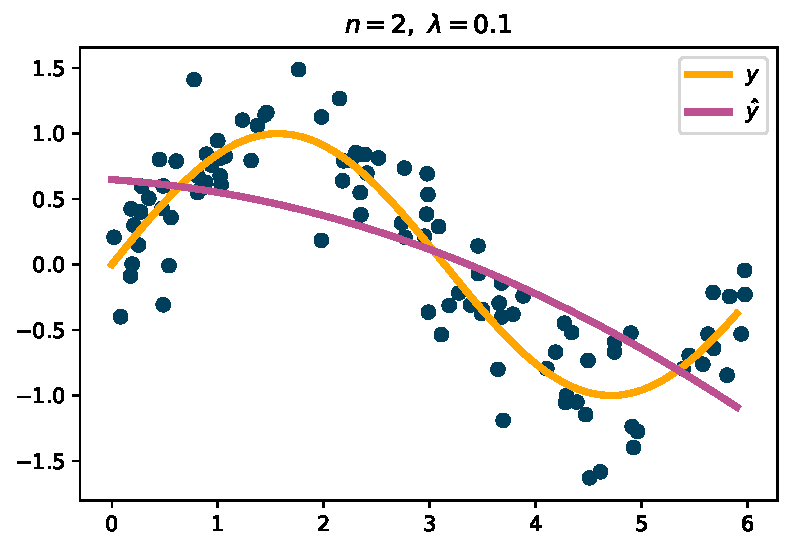
\includegraphics[width=0.47\linewidth]{figures/kernels-sin-poly-2.pdf}
\hfill
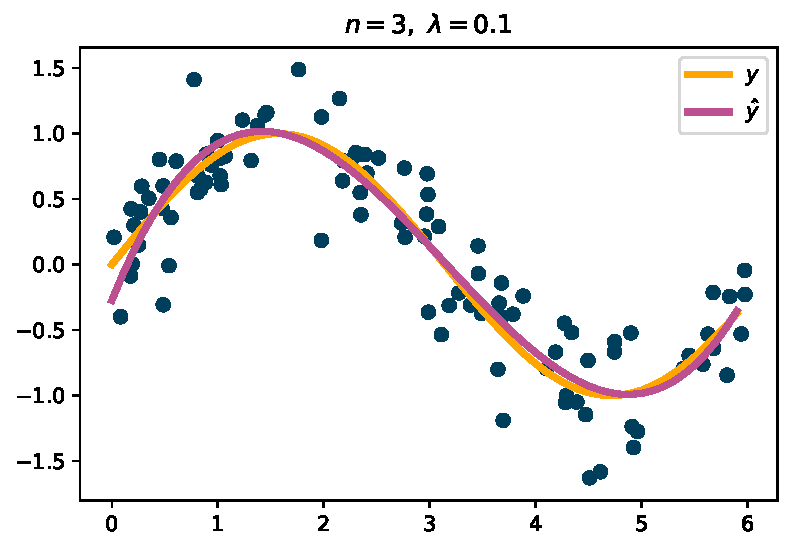
\includegraphics[width=0.47\linewidth]{figures/kernels-sin-poly-3.pdf}
}
\caption{Kernelized ridge regression with polynomial kernel on one-dimensional data. Choice of hyper-parameter of the kernel can greatly influence the degree of fit.}
\label{fig:kernels-poly}
\end{figure}

\begin{figure}
\centering{
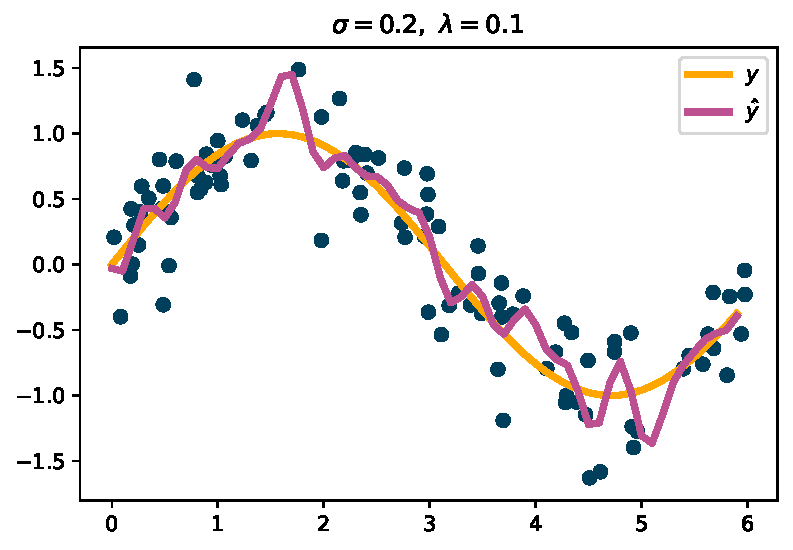
\includegraphics[width=0.47\linewidth]{figures/kernels-sin-rbf-02.pdf}
\hfill
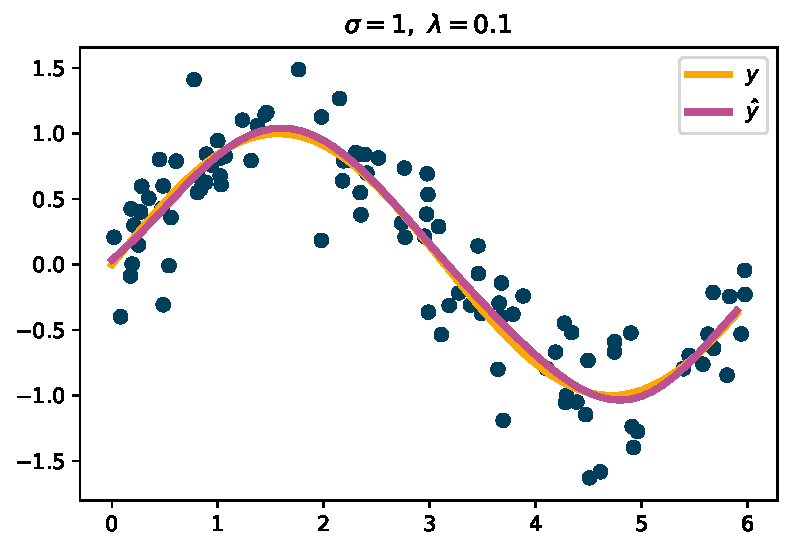
\includegraphics[width=0.47\linewidth]{figures/kernels-sin-rbf-10.pdf}
}
\caption{Wrong choice of hyperparameters can lead to overfitting, as shown in the plots of regression on one-dimensional data set with Gaussian kernel.}
\label{fig:kernels-poly}
\end{figure}

\subsection*{Support Vector Machines}

Support vector machines are, in essence, linear classifiers that infer separating hyper-planes with maximal margins to the neighboring data points. We here derive the formulation of this classifier, show how to its power with a kernel trick, and describe extension for non-linearly separable cases. We also derive the formulation for support vector machines using hinge loss.

\subsubsection*{The Large Margin Principle}

\begin{figure}[htbp]
\centering{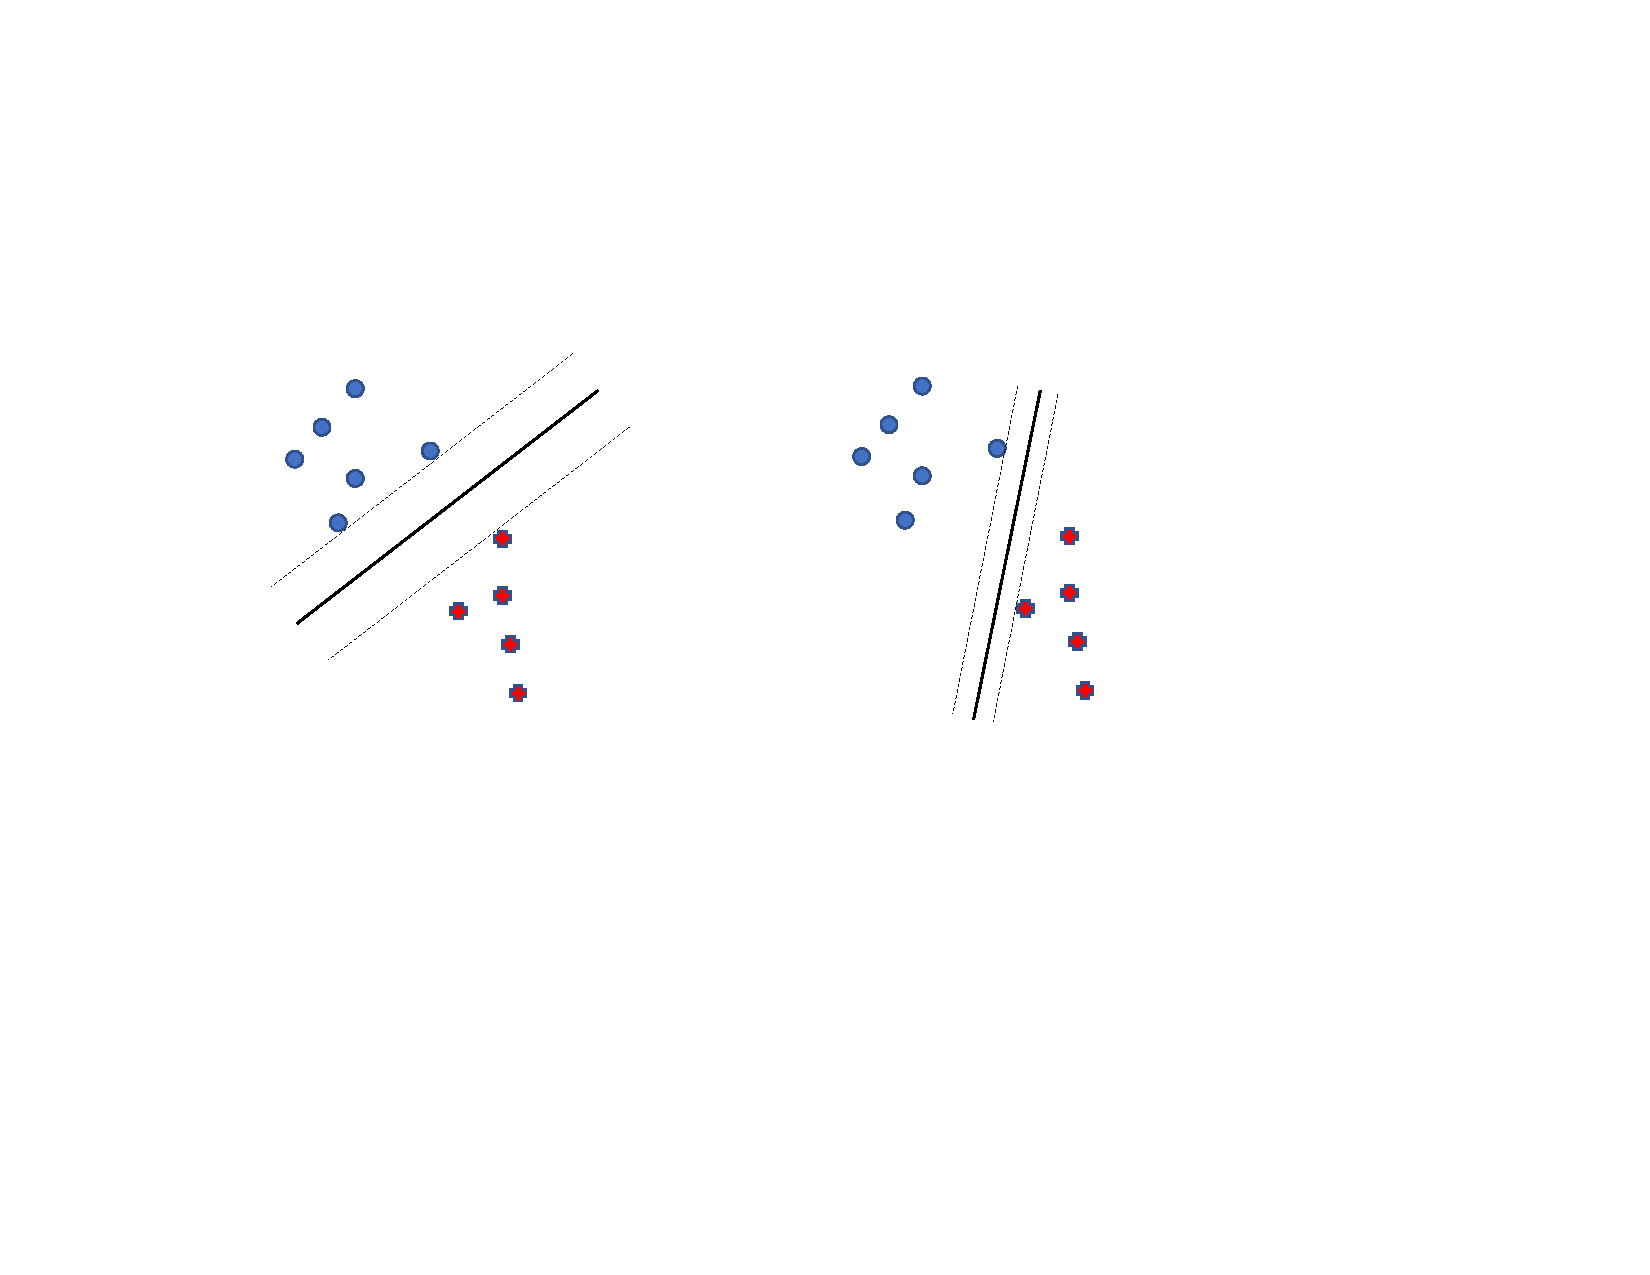
\includegraphics[width=12cm]{figures/kernels-margin.pdf}}
%TODO
\caption{A separating hyper-plane with large (left) and small margin (right).}
\label{fig:svm-lin-sep}
\end{figure}

Consider a binary classification problem, with $y=\pm 1$, where data instances of the two classes are linearly separable. Our aim is to define a separating hyper-plane that splits the feature space so that the margin between the closest positive and the closest negative data instance is the largest~\ref{fig:svm-lin-sep}. Intuitively, a large margin would steer us from overfitting and may yield best accuracy on yet unseen data. Let us denote the margin with $\gamma$. We would therefore like to find $\vect{w}$ that defines the direction of a separating hyper-plane $\vect{w}^\tr\vect{x}+w_0=0$, where $w_0$ is the intercept, with largest margin $\gamma$. With no loss of generality, let us choose $w$ so that the data points on the margin are one unit away from separating hyper-plane. The equations for the margins are thus:
\begin{align*}
\vect{w}^\tr\vect{x}+w_0 &= 1 \\
\vect{w}^\tr\vect{x}+w_0 &= -1 \\
\end{align*}
Consider now a point $\vect{x}$ on one margin and its projection $\vect{x}_\perp$ accross separating hyperplane to the other margin:
$$ \vect{x} = \vect{x}_\perp + 2\gamma {\vect{w}\over\norm{\vect{w}}} $$
Using the equations of the margin, so that $\vect{w}^\tr\vect{x}+w_0 = 1$ and $\vect{w}^\tr\vect{x}_\perp+w_0 = -1$, we obtain:
$$ \vect{w}^\tr\left(\vect{x}_\perp + 2\gamma {\vect{w}\over\norm{\vect{w}}}\right) + w_0=1, $$
$$ \vect{w}^\tr\vect{x} + w_0 + 2\gamma {\vect{w}^\tr\vect{w}\over\norm{\vect{w}}}
= 1, $$
$$ -1 + 2\gamma {\vect{w}^\tr\vect{w}\over\norm{\vect{w}}}
= 1, $$
and finally, considering $\vect{w}^\tr\vect{w}=\norm{\vect{w}}^2 $,
$$ \gamma = {1\over\norm{\vect{w}}} $$
To maximize the margin, we need to minimize the length of $\vect{w}$. Formally, and considering that all data points in our linearly separable classification problem have to lie on or outside the margin, we therefore want to opimize
$$\min_{\vect{w},w_0} {1\over 2}\norm{w}^2\ s.t.\ y_i(\vect{w}^\tr \vect{x}_i+w_0)\geq 1,\ i=1\ldots N$$
For convenience, we have added $1\over 2$ and are optimizing the squared norm instead of the norm, which, of course, should be mathematically more convenient and leads to the same solution. We can now use the method of Lagrange multipliers to find the minima of our criteria function that succombs to the set of constrains. The primal Lagrangian is:
$$ L(\vect{w},w_0,\vect{\alpha})={1\over 2}\norm{w}^2 - \sum_{i=1}^N \alpha_i [y_i(\vect{w}^\tr \vect{x}_i+w_0)-1] $$
where $\alpha_i\geq 0$ are Lagrange multipliers. Optimal value of parameters that define the separating hyper-plane is where the gradient of the Lagrangian is zero:
\begin{align*}
\nabla L &= \pd{L}{\vect{w}} \\
&= \vect{w} - \sum_{i=1}^N \alpha_i y_i \vect{x}_i = 0
\end{align*}
Therefore,
\begin{equation}
\vect{w}=\sum_{i=1}^N \alpha_i y_i \vect{x}_i
\label{eq:svm-w}
\end{equation}
Separating hyperlane is defined through a normal vector that is a weighted sum of vectors that define our training data instances!

Similar holds for $w_0$,
$$ \pd{L}{b}=-\sum_{i=1}^N \alpha_i y_i = 0 $$
and hence
$$ \sum_{i=1}^N \alpha_i y_i = 0 $$

We now insert the values of our optimal parameters back to the Lagrangian:
\begin{eqnarray*}
L & = & {1\over 2} \left(\sum_{i=1}^N \alpha_i y_i \vect{x}_i \right) \left(\sum_{j=1}^N \alpha_j y_j \vect{x}_j \right) - \left(\sum_{i=1}^N \alpha_i y_i \vect{x}_i \right) \left(\sum_{j=1}^N \alpha_j y_j \vect{x}_j \right) - \sum_{i=1}^N \alpha_i y_i + \sum_{i=1}^N \alpha_i \\
& = & \sum_{i=1}^N \alpha_i - {1\over 2}\sum_{i=1}^N\sum_{j=1}^N \alpha_i\alpha_j y_i y_j \vect{x}_i\vect{x}_j
\end{eqnarray*}
Support vector classifier is then defined through the following optimization problem:
\begin{eqnarray*}
{\rm maximize} && L(\alpha) = \sum_{i=1}^N \alpha_i - {1\over 2}\sum_{i=1}^N\sum_{j=1}^N \alpha_i\alpha_j y_i y_j \vect{x}_i\vect{x}_j \\
{\rm subject\ to} && \sum_{i=1}^N y_i\alpha_i = 0, \\
&& \alpha_i\geq 0,\ i=1,\ldots, N
\end{eqnarray*}
The problem of finding the separating hyper-plane with maximal margin thus translates to quadratic programming, for which a standard solver can be used.

At this stage, notice that finding $\vect{\alpha}$ through quadratic programming provides us the weights $\vect{w}$ (see Eq.~\ref{eq:svm-w}) and consequently provides for $b$. Notice that the solution of a quadratic programming problem, that is, the vector $\vect{\alpha}$ is typically sparse. That is, most $\alpha_i$ will be zero. That is, the weights $\vect{w}$ will be defined by only a small number of input data instances. These data instances are those that define the margin and are called {\em support vectors}. The support vectors are, therefore, training data instances for which $\alpha_i>0$.

The decision rule for classification of data instance $\vect{x}$ to the positive class ($y=1$) is
$$ \vect{w}^\tr\vect{x}+b\geq0 $$
and if we substitute for $\vect{w}$ we obtain:
$$ \sum_{i=1}^N \alpha_i y_i\vect{x_i}^\tr \vect{x} + b \geq 0 $$
Notice that in essence we do not need to compute the weights $\vect{w}$ for classification. All we need is to remember the instances for the training data set and compute the scalar product between training data instances and the vector the represents data instance to be classified. We can notice that in the quadratic programming formulation, where we solve for $\vect{\alpha}$, its dependency on the training data is again expressed through the scalar product $\vect{x}_i^\tr\vect{x}_j$.

\subsubsection*{Support Vector Machines and Kernel Trick}

Consider a data set with linearly non-separable classes (Fig.~\ref{fig:svm-circle}, left panel), and a transformation $\Phi(\vect{x})=\langle x_1^2, x_2^2, \sqrt{2}\ x_1 x_2\rangle$ that takes each two-dimensional data instance and transforms it into a latent space with three dimension. The transformed data set becomes linearly separable (Fig.~\ref{fig:svm-circle}, right panel). If $\vect{x}$ and $\vect{x}'$ are two vectors in original space, what is their dot product $\Phi(\vect{x})\Phi(\vect{x}')$ in transformed space?
\begin{align*}
\Phi(\vect{x})\Phi(\vect{x}') & = \langle x_1^2, x_2^2, \sqrt{2}\ x_1 x_2\rangle^\tr \langle x_1'^2, x_2'^2, \sqrt{2}\ x_1' x_2'\rangle \\
& = x_1^2 x_1'^2 + 2 x_1 x_2 x_1' x_2' + x_2^2 x_2'^2 \\
& = (x_1 x_1' + x_2 x_2') \\
& = (\vect{x}^\tr \vect{x}')^2
\end{align*}

\begin{figure}[htbp]
\centering{
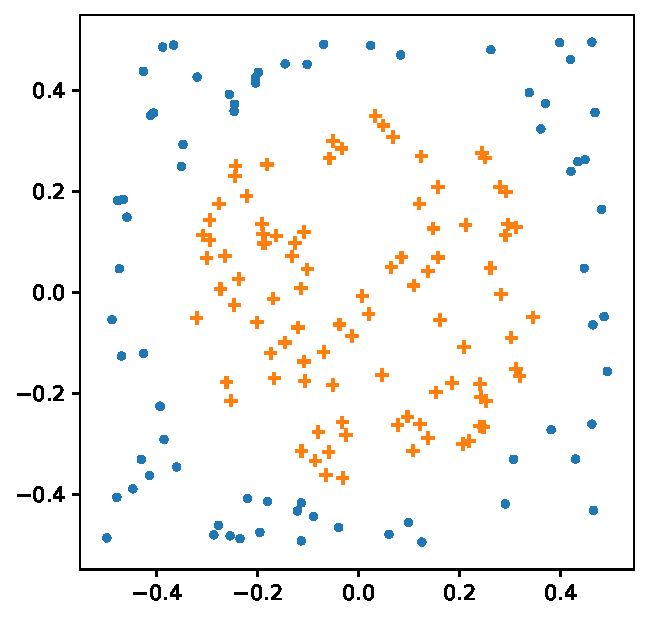
\includegraphics[width=0.49\linewidth]{figures/kernels-circle.pdf}
\hfill
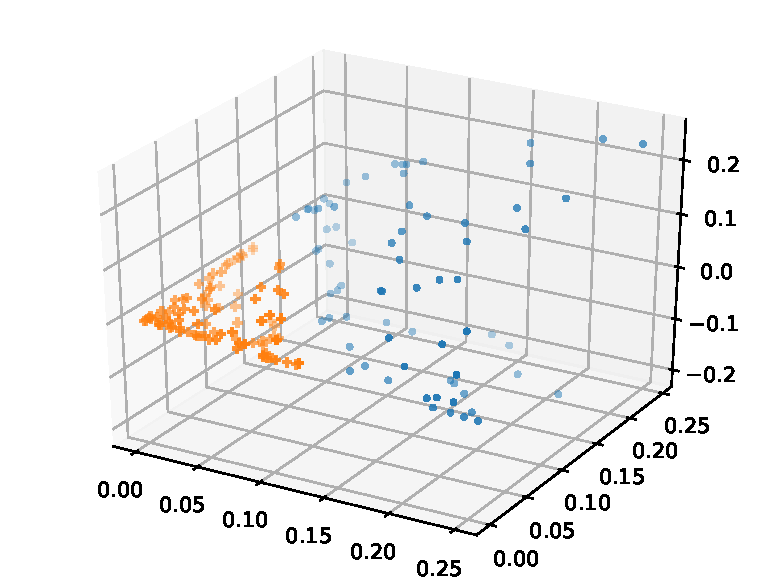
\includegraphics[width=0.49\linewidth]{figures/kernels-circle-3d.pdf}}
\caption{A two-feature binary classification data set (left), where the data points of different classes are not linearly separated. The same data set, where each point $\vect{x}$ was transformed through $\Phi(\vect{x})$, so that $\Phi(\vect{x})=\langle x_1^2, x_2^2, \sqrt{2}\ x_1 x_2\rangle$ (right).}
\label{fig:svm-circle}
\end{figure}

So, if, instead of using a dot product between two vectors $\x^\tr\x'$ in formulation of SVM, we can replace it with a $\kappa(\x,\x')=(\x^\tr \x')^2$. This substitution is called a kernel trick. The kernel trick avoids the explicit mapping that is needed to, say, get a linear model to learn a nonlinear function or decision boundary. For all $\x$ and $\x'$ in the input space, certain functions $\kappa(\x, \x')$ can be expressed as an inner product in another space. The function $\kappa$ is referred to as a kernel or a kernel function. Notice that the kernel trick allows us never to transform the data to the latent space, that is, never to use the transformation function $\Phi(\vect{x})$. In this way, the latent space could, in principle, have infinite dimensions, yet all we need is to compute the scalar product in this space. For any kernel, there is a corresponding function that transforms the data from original space to latent space, and there are some kernels where the required dimensionality of latent space is infinite. We will discuss various kernel functions and their properties a bit later in this chapter.

\begin{figure}
\centering{
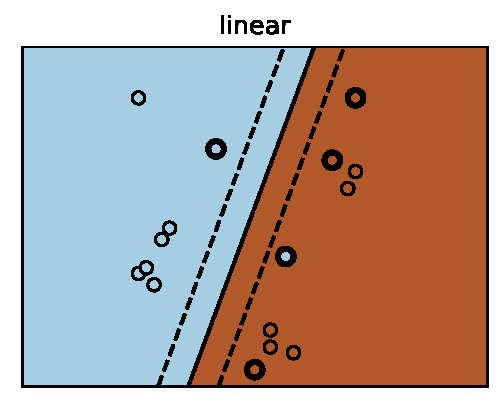
\includegraphics[width=0.32\linewidth]{figures/kernels-svm-linear.pdf}
\hfill
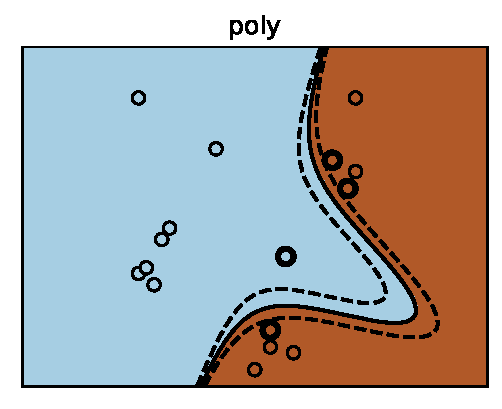
\includegraphics[width=0.32\linewidth]{figures/kernels-svm-poly.pdf}
\hfill
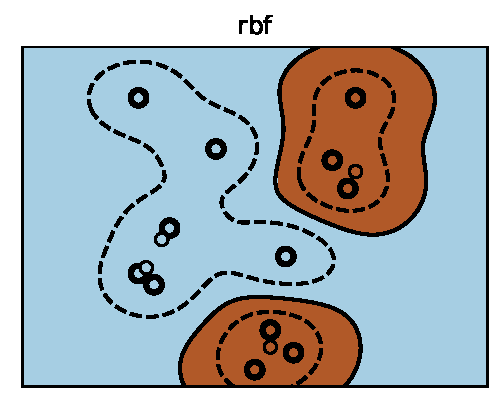
\includegraphics[width=0.32\linewidth]{figures/kernels-svm-rbf.pdf}
}
\caption{Classification in two-dimensional feature space shows decision boundaries of support vector machines with linear, polynomial ($n=3$), and Gaussian kernel. Double-circled data points are support vectors. Code for figures by Gaël Varoquaux.}
\label{fig:kernels-poly}
\end{figure}

\subsubsection*{Non-Linearly Separable Data}

If the data is not linearly separated, which is expected from any real data that contains some noise, the support vector machine that we have defined so far does not have any solution. For such cases, we need to introduce slack variables $\xi_i\geq 0$ such that slack is zero if the data instance is on or inside the correct margin boundary, or the slack is positive and equal to the distance to the corresponding margin. Notice that if $0<\xi_i\geq 1$ the point lies inside the margin, but on the corre side of decision boundary. To solve for this problem, we replace the hard constrains with {\em soft margin constraints} with the new objective, where, as before, we would like to maximize the margin with minimal use of slack:
$$ \min_{\vect{w},w_0,\vect{\xi}} {1\over 2}\norm{w}^2+C\sum_{i=1}^N\xi_i\ \ s.t.\ \xi_i\geq 0,\ y_i(\vect{w}^\tr \vect{x}_i+w_0)\geq 1-\xi_i,\ i=1\ldots N$$
The corresponding Lagrangian is
$$ L(\vect{w},w_0,\vect{\alpha})={1\over 2}\norm{w}^2 + C\sum_{i=1}^N\xi_i - \sum_{i=1}^N \alpha_i [y_i(\vect{w}^\tr \vect{x}_i+w_0)-1+\xi_i] -\sum_{i=1}^N\mu_i\xi_i$$
After computing the corresponding gradients and replacing the results in the primal Lagrangian, the dual form of Lagrangian is the same as before,
$$ \sum_{i=1}^N \alpha_i - {1\over 2}\sum_{i=1}^N\sum_{j=1}^N \alpha_i\alpha_j y_i y_j \vect{x}_i\vect{x}_j $$
with the only exception of a box constrain $0\leq\alpha_i\leq C$. Notice that the parameter $C$ is a regularization parameter that controls the number of errors we are willing to tolerate on the training set. This parameter is commonly defined as $C=1/(\nu N)$, where $0<\nu\leq 1$ is the fraction of misclassified points we allow during the training phase. This version of the algorithm is called $\nu$-SVM classifier.

\subsubsection*{Multi-Class Classification}

We have defined support vectors classifiers for supervised learning on binary classification data. Unlike some other approaches, like softmax for logistic regression, SVMs do not have a natural extension that would be appropriate to treat multi-class data. Standard approaches that solve multi-class problems through inference of a set of binary classifiers include a one-versus-all approach and one-versus-one approach. However, the problem to use them is that SVM, in its original formulation, is not a probabilistic classifier.

\subsubsection*{Choosing the Value of Hyper-Parameters}

Regularization parameters like $C$ and $\nu$ are parameters of the algorithm, that is, hyper-parameters that need to be set before the inference of the model. To search for the most appropriate value, we can use approaches such as the search over a fixed set of parameters and estimating their appropriateness through cross-validated accuracy on the training data. We then use the parameter value with the highest estimated accuracy to infer the model from the entire training set.

\subsubsection*{Hinge Loss}

An alternative derivation of support vector machine comes from the utility of {\em hige loss}, a variant of a loss function for binary classification, defined as:
$$ L_{\rm hinge}(y, \eta) = \max(0, 1-y\eta) = (1-y\eta)_{+} $$
Here, $\eta=f(\x)=\vect{w}^\tr x + w_0$ can be regarded as ``confidence'' in choosing label $y=1$. The overall objective is again to maximize the margin while minimizing the loss, therefore:
$$ \min_{\vect{w},w_0}{1\over 2}\norm{\vect{w}}^2 + C\sum_{i=1}^N(-y_i f(\vect{x}_i))_{+} $$
This objective function is non-differentiable because of the max term. We can replace this term with slack variables, and request in the revised objective that the slack is minimized. The new objective function 
$$ \min_{\vect{w},w_0,\vect{\xi}} {1\over 2}\norm{w}^2+C\sum_{i=1}^N\xi_i\ \ s.t.\ \xi_i\geq 0,\ y_i(\vect{w}^\tr \vect{x}_i+w_0)\geq 1-\xi_i,\ i=1\ldots N$$
is exactly the same as the one derived above, in the section on the treatment of non-linearably separable data.


\subsection*{Kernelized $k$-Nearest Neighbors}

$k$-nearest neighbor algorithms are based on distance, that is, they find the observations closest to the one we are predicting for. If using an Euclidean distance, this can be expressed in terms of inner products 
%
$$\lvert\lvert x, x' \rvert\rvert^2 =  \lvert\lvert x \rvert\rvert^2 + \lvert\lvert x' \rvert\rvert^2 - 2 \langle x, x'\rangle  =  \langle x, x\rangle^2 + \langle x', x'\rangle^2 - 2 \langle x, x'\rangle.$$
%
Thus, we can replace these dot products with a kernel, and in this way perform $k$-nearest neighbors in the feature space of a chosen kernel.

\subsection*{Support Vector Machines Regression}
% This is basically my review of 14.5.1; maybe some additional comments

Here, we motivate SVM with the problem of kernelized ridge regression, and actually with other approaches discussed so far that use the kernel trick, where the solution is not sparse. More precisely, the solution of kernelized ridge regression $\hat{\beta} = \sum \alpha_i \x_i$ and subsequently the predictions  $\hat{y}(x')  = \sum \alpha_i \kappa(\x',\x_i)$ depend on all training observations.

A key idea of SVMs is to introduce sparsity through the loss function. Vapnik proposed the \emph{epsilon insensitive loss function}:

$$L_\epsilon(y, \hat{y}) = |y-\hat{y}| - \epsilon\ {\rm if}\ |y-\hat{y}| \geq \epsilon\ {\rm and}\ 0\  {\rm otherwise}.$$
Basically, anything that has an absolute error less than $\epsilon$ is not penalized. The objective function we want to minimize is then

$$J = C\sum L_\epsilon(y_i, \hat{y}_i) + \frac{1}{2}\lvert\lvert \beta \rvert\rvert^2,$$
%
where $\hat{y}_i = f(\x_i) = \beta^T \x_i + \beta_0$ and $C = \frac{1}{\lambda}$ is a regularization constant.

This optimization problem is non-differentiable because of the absolute value in the loss function. Typically, it is reformulated as a constrained optimization problem by introducing slack variables $\xi$:

\begin{align*}
y_i - f(\x_i) & \leq + \epsilon + \xi_i^+, \\
y_i -  f(\x_i) & \geq - \epsilon - \xi_i^-.
\end{align*}

Now we can reformulate the objective function.

$$J = C\sum (\xi_i^+ + \xi_i^-) + \frac{1}{2}\lvert\lvert \b \rvert\rvert^2.$$
%
This is a quadratic function of $\b$ and we need to minimize it, subject to the above constraints and $\xi_i^+ \geq 0$, $\xi_i^- \geq 0$. Standard quadratic programming black-box solvers can be used.

If it is not immediately clear what we did with the slack variables: First, we deliberately put the  $f(\x_i)$ on the left-hand side of the inequality constraints above. This is to illustrate the fact that for observations that we can fit within $\epsilon$, the constraint will immediately be true, and both $\xi_i$ can be 0. For all other observations, one of the inequality constraints will be violated, but not both. So, one of the slack variables will be 0, and the other will be exactly the amount the fit exceeds $\epsilon$. This is what forces the $f(\x_i)$ as close to $y_i$ as possible, in the absolute sense; the only way to make $\xi_i$ as close to 0 as possible, again, in the absolute sense, is to make the $f(x_i)$ as close to $y_i$ as possible. That is, in the optimal solution, the sum of $\xi$ will be exactly the total sum of all exceedances of $\epsilon$), so by minimizing the one, we minimize the other. But we got rid of the absolute term.

The solution of the above optimization problem \citep{2012-Murphy} has, not surprisingly, the form
$$\hat{\b} = \sum_i \alpha_i \x_i,$$
%
where $\alpha_i \geq 0$. Notice that this solution is typically sparse, as most $\alpha_i = 0$. The $\x_i$ where $\alpha_i > 0$ are again called \emph{support vectors}. We should emphasize that the sparseness comes from the objective function ($\epsilon$). In practice, and depending on training data, we sometimes do get unlucky as it turns out that most $x_i$ from the training data are support vectors.

SVM regression is typically solved in its dual form. The form above is the primal form. The two forms are the same as the optimization problem is convex. The dual formulation is also where the result comes that the solution is a linear combination of observations, very similar to kernelized ridge regression.

As with kernelized ridge regression, the prediction for a new observation is
\begin{align*}
\hat{y}(x') & = \hat{\beta}_0 + x'^T\hat{\beta} \\
& = \hat{\beta}_0 + x'^T\sum \alpha_i x_i \\
& = \hat{\beta}_0 + \sum \alpha_i x'^Tx_i \\
& =  \hat{\beta}_0 + \sum \alpha_i \kappa(x', x_i)
\end{align*}
So, we can also use the kernel trick here and do SVM regression in a feature space determined by the choice of kernel.

\section*{Kernel Density Estimation}

Here, we will discuss on a substantially different kind of kernels, the so-called {\em smoothing kernels}. We will use the smoothing kernels to create non-parametric density estimates $p(\x)$, as well as for creating generative models for classification and regression of the form $p(y,\x)$.

A smoothing kernel is a one-argument function that satisfies the following properties:
$$ \int \kappa(x)dx = 1, $$
$$ \int x\kappa(x)dx = 0, $$
$$ \int x^2\kappa(x)dx > 0. $$

A simple example of a smoothing kernel is a {\em Gaussian kernel},
$$ \kappa(x)={1\over (2\pi)^{1\over 2}} e^{-x^2/2} $$
and we can control the width of the kernel by introducing a {\em bandwidth} parameter $h$:
$$ \kappa_h(x)={1\over h}\kappa{x\over h} $$
We can generalize this kernel to vector-valued inputs by defining an RBF kernel:
$$ \kappa_h(\x) = \kappa_h(\norm{\x}).$$

Kernel density estimators are different from, say, Gaussian mixture models, a parametric density estimator that requires speficying $K$ prototypes. An alternative is to allocate one cluster center per data point, so that the kernel density estimator, also called the {\em Parzen window density estimator} becomes
$$ \hat{p}(\x) = {1\over N}\sum_{i=1}^N \kappa_h(\x-\x_i).$$

The advantage of kernel density estimator over the parametric models is no need for model fitting and no need to pick the prototypes. However, we need to tune for the bandwidth, which can be performed by internal cross-validation. Notice also that the choice of $h$ influences the bias-variance tradeoff. More smoothing decreases bias but increases variance, less smoothing decreases variance but increases bias. The optimal point is somewhere in between. 


% \begin{itemize}
% \item What smoothing kernels are (14.7.1)
% \item Kernel density estimation and mention of histogram (14.7.2) NOTE: Murphy doesn't have an example of the important underlying principle - it's all about the bias-variance tradeoff. More smoothing decreases bias but increases variance, less smoothing decreases variance but increases bias. The optimal point is somewhere in between. You may want to refer to Wasserman's All of statistics: 20.1 (bias-variance tradeoff), 20.2 (histograms), 20.3 (KDE)
% \item OPTIONAL (kNN and kernel regression (14.7.3-4)
% \item LOESS (locally weighted regression) (14.7.5); this is pretty much state-of-the-art for 1D smoothing
% \end{itemize}

\printbibliography[heading=subbibliography]
\end{refsection}




\end{document}
